\documentclass[11pt]{article}
%%%%%%%%%%%%%%%%%%%%%%% Don't change anything in here. This space is called the preamble, it is where you tell the computer to load the proper LaTeX packages to perform the math and formatting desired. 

\usepackage{physics} 
\usepackage{siunitx} 
\usepackage{enumerate} 
\usepackage{pgfplots}
\usepackage{float}
\usepackage{ucs}
\usepackage{caption}
\usepackage{subcaption}
\usepackage[utf8]{inputenc}
\usepackage{pgfplotstable}
\usepackage{tikz,pgfplots}
\usepackage{csvsimple} %convert csv and tsv into latex tables
\usepackage{amsmath}  %I added this so that you can use the align tool for equations!
\usepackage{wasysym} %This package allows you to put emojis in your paper!!!!
	%wasysym: \smiley{} \frownie{} see http://milde.users.sourceforge.net/LUCR/Math/mathpackages/wasysym-symbols.pdf for list of most symbols available in this package
	\makeatletter
\def\rightharpoonupfill@{%
  \arrowfill@\relbar\relbar\rightharpoonup} 
\def\leftharpoondownfill@{%
  \arrowfill@\leftharpoondown\relbar\relbar}

\usepackage{graphicx}
\graphicspath{ {./images/} }
\usepackage{hyperref}

\usepackage{lscape}
\usepackage[toc]{appendix}


% Package to insert code in LaTeX
\usepackage{listings}
\usepackage{color}
\definecolor{dkgreen}{rgb}{0,0.6,0}
\definecolor{gray}{rgb}{0.5,0.5,0.5}
\definecolor{mauve}{rgb}{0.58,0,0.82}
\lstset{frame=tb,
  language=Bash,
  aboveskip=3mm,
  belowskip=3mm,
  showstringspaces=false,
  columns=flexible,
  basicstyle={\small\ttfamily},
  numbers=none,
  numberstyle=\tiny\color{gray},
  keywordstyle=\color{blue},
  commentstyle=\color{dkgreen},
  stringstyle=\color{mauve},
  breaklines=true,
  breakatwhitespace=true,
  tabsize=3
}

	
\usepackage{geometry}
 \geometry{
 a4paper,
 total={170mm,257mm},
 left=30mm,
 right=30mm,
 top=20mm,
 }

\pgfplotsset{compat=1.14}
%%%%%%%%%%%%%%%%%%%%%%%%% Again, Don't change anything Above %%%%%%%%%%%%%%%%%%%%

\begin{document}
\title{Computational Microbial Genomics \\\ Report  \\\  A.Y. 2021-2022 \\\ 

A Study to Identify Geographical Signatures in a Pangenome from Human Gut Microbiome} %Title  
\author{\begin {tabular}{c c c}
Submitted to: Prof. Dr. Nicola Segata \\\
\linespread{5}
Submitted by: 
              Surbhi Malhotra,  
              Surya Hembrom, 
              Annalisa Xamin
\end{tabular}}

\date{11 April 2022}  % This will automatically put today's date in the report
\begin{figure}
    \centering
    
\includegraphics[width=0.4\columnwidth]{logouni.png}
\end{figure}
\maketitle  %this command makes the title
%%%% to use this template, please copy-paste the entire thing into a new document and save it so you have it!
\vspace*{\fill}
\centerline{\textit{University of Trento - Via Sommarive 9, 38123 Povo (TN), Italy}}
\thispagestyle{empty}


\newpage
%%%%% If you want to omit something in this lab, place a % sign to the left of it and it won't show up on the lab, like this line!
\tableofcontents

\thispagestyle{empty}
\newpage
\setcounter{page}{1}


\newpage
%%%%%%%%%%%%%%%%%%%%%%%%%%%%%%%%%%%%%%%%%%%%%%%%%%%%%%%%%%%%%%%%%%%%%%%%%%%%%%%%%%%%%%

\section{Introduction} 
Human gut microbiome is a complex environment, promoting several microbial species and strains survive and has been related to etiology of important human diseases across different populations and impacts overall human health\cite{Nayfach_2019, Armour2019}. The gut of healthy and diseased individuals vary due to changes in gut microbiome and presence of various microbial species and strains and their differential functioning of genes \cite{Armour2019}. Currently, Metagenome-assembled-genomes (MAGs) have led to rapid advancement in identification of various unprecedented gut microbial species and their strains with no or unfeasible standard lab-culturing techniques, or no high-quality reference genomes \cite{Jin2022}, even bypassing tedious lab-isolation and lab-culturing of hundreds of samples \cite{Watson2021.04.02.438222, Nayfach_2019} through affordable sequencing technologies \cite{Asnicar2020}. The MAGs are constructed from contigs, which are formed by assembly of sequencing reads, through a binning process of single metagenome or several co-assembled metagenomes depending on nucleotide frequency, co-abundance, abundance (genes binned on co-abundance criteria are known as co-abundance gene groups (CAGs) \cite{Nielsen2014}) and, or co-variation of abundance among several sample groups \cite{Nayfach_2019} presumed on \textit{k}-mers\cite{Setubal2021}. The quality control of MAGs is crucial for recognition and removal of potential contaminants, identification of marker genes, and contiguity and completeness of metagenomes\cite{Nayfach_2019} before any comparative genomic analyses.\\
In this study we aimed to understand if human gut microbiome from different individuals exhibit any geographical signatures. For this, we examined high quality single taxon uSGB (unknown Species-level genome bin; SGB comprises either MAGs or MAGs and isolates aggregated from closely related strains of a species based on phylogenetics \cite{Asnicar2020}) from individuals with no to varied health conditions from different countries. We also investigated the degree of within-taxon proximity of MAGs in this SGB to a known bacterial \textit{Clostridium} species genome. For this, we determined the phylogenetic relationship of these SGBs to \textit{Clostridium} spp. isolate. We even estimated, the proportions of core and accessory genes of all the SGBs to envisage any underlying pangenomic-level dynamics. Lastly, we investigated if these SGBs were conducive to specific disease-related pathogenicity in diseased or healthy individuals.   

\section{Materials and Methods}
\subsection{Sample data}

We studied samples from project SGB6179 (uSGB) with 26 MAGs and 1 uncultured, whole genome shotgun sequenced \textit{Clostridium} spp. isolate UMGS222. Out of which, 24 MAGs were human gut microbiome sampled from stools of 18 healthy, 3 diseased (1 with Type2 Diabetes: T2D, 1 with colorectal cancer: CRC, and 1 with HBV: Hepatitis B + HDV: Hepatitis D + cirrhosis) and 3 unknown health conditions. 2 MAGs were not described in metadata but are related to human stool sampled from gut microbiome studies by Nayfach et al., 2019 \cite{Nayfach_2019}, and Nayfach et al., 2020\cite{Shi2020}. Including healthy and unknown health conditions, we had 21 disease controls. All MAGs and isolate genome were checked for completeness of $>$90\% and redundancy $<$5\%. (see Appendix - Table \ref{Table:SGB_metadata}, \ref{Table:SGB_metadata2}, \ref{Table:SGB_bin_data}). 

\subsection{Genome annotation}
Genome annotation is labelling the CDS and intergenic regions inside the assembled genome. We annotated the MAGs and isolate fasta files with PROKKA, which incorporates several bioinformatics tools to acquire fast and reliable annotations of genomic bacterial sequences \cite{Seemann2014}, with the following commands: 
\newpage
\begin{lstlisting}
prokka --kingdom Bacteria --outdir prokka\_out --locustag L --prefix MAG\ filename
\end{lstlisting}
wherein --kingdom represents the bacterial kingdom used for genome annotation, --locustag represents locustag, an identifier systematically attached to each gene. Following annotation, we extracted the number of CDS regions (in .txt files), hypothetical proteins and known protein (in .tsv files) per sample with custom bash scripts. 

\subsection{Pangenome analysis}
Clustering of conspecific genomes with high confidence protein sequences with substantial amino acids identity engender pangenomes \cite{Almeida2019}. Pangenome analysis identifies the cumulative curve of genetic variability attributive of a given species with increase in individual genomes sequenced\cite{Muzzi2011,Nguyen2015}. We input the genome annotations (.gff files) from PROKKA into Roary\cite{Page2015} (using GNU parallel \cite{tange_2022_6213471}) to retrieve microbial species' pangenome.\\
We did two runs of analyses with Roary:
\begin{enumerate}
\item Based on rapid Blastp alignment to check the presence or absence of the accessory genes.
\item Based on MAFFT\cite{Katoh2002} and PRANK\cite{Lytynoja2013} alignments of the core genes.
\end{enumerate}

\subsubsection{Based on Blastp alignments for presence or absence of accessory genes}
We ran Roary with parameters -i for 95\% identity cutoff for Blastp alignment (as 95\% performed well, Figure \ref{fig:roary1_1}) and -cd for 95\% minimum threshold for all isolates to contain a gene to be classified as core gene, with default thread 1.
\begin{lstlisting}
roary *.gff -f roary_out -i 95 -cd 95
\end{lstlisting}

We processed the Roary alignment outputs for the presence/absence count of the accessory genes with Roary-inbuilt R-enabled python script roary\_plots.py (\url{https://raw.githubusercontent.com/sanger-pathogens/Roary/master/contrib/roary_plots/roary_plots.py})
with the following commands:
\begin{lstlisting} 
python3 roary_plots.py accessory_binary_genes.fa.newick gene_presence_absence.csv
\end{lstlisting}
We obtained:
\begin{enumerate}
\item Pangenome frequency plot
\item Presence and absence matrix plot against the tree
\item Pangenome pie-chart (core, soft core, shell and cloud genes)
\end{enumerate}

We used Roary-inbuilt R script create\_pan\_genome\_plots.R \url{https://github.com/sanger-pathogens/Roary/blob/master/bin/create_pan_genome_plots.R} to understand the dynamics of pangenome. We retrieved the total number of genes under four different categories i.e., core, soft, shell, and cloud genes forming the pangenome.
\newline
We obtained plots with:
\begin{enumerate}
\item The number of Blastp hits with different percentage identity.
\item The number of conserved and total genes with increase in the number of genomes.
\item The number of unique and new genes with increase in the number of genomes.
\end{enumerate}

\subsubsection{Based on alignments of the core genes}
We ran Roary for multiFASTA alignment of core genes\cite{Page2015}. with additional parameters -e for slow and accurate alignment with inbuilt PRANK and -n for fast alignment with inbuilt MAFFT using default thread 1.
\begin{lstlisting}
roary *.gff -f roary_out_align -e -n -i 95 -cd 95
\end{lstlisting}

We did further alignment analyses using the same create\_pan\_genome\_plots.R and roary\_plots.py scripts.

We compared the results from first run of Roary to its second run  the second analysis. These results are eminent for downstream analyses such as phylogenetic tree reconstruction and SNPs identification\cite{Farrah2019}.

\subsection{Taxonomic characterisation}
We taxonomically characterised the MAGs with PhyloPhlAn\cite{Asnicar2020}.

\begin{lstlisting}
phylophlan_metagenomic -i phylophlan_input -o phylophlan_output --nproc 4 -n 1 --database_update -d CMG2122 --verbose -e .fa 
\end{lstlisting}
wherein we used parameters --nproc for 4 number of CPUs; -n for number of best hit within each MAG matching the database to retain, -d for database CMG2122 with --database\_update for database updation, -e for fasta format (.fna or .fa). \\

\subsection{Phylogenetic structure}
We visualized the phylogenetic trees from MAGs and isolate with \href{https://itol.embl.de/}{Interactive Tree Of Life(iTOL)} v6, an online tool for the display, annotation and management of phylogenetic and other trees\cite{Letunic2021}.
We reconstructed phylogenetic trees from two different Roary analyses: 
\begin{enumerate}
\item \textbf{Phylogenetic tree based on presence/absence of accessory genes (Roary)}: \\Uploaded  accessory\_binary\_genes.fa.newick to the iTOL.
\item \textbf{Phylogenetic tree based on core genes alignment (Roary with additional -e and -n parameters)}:  Using FastTree\cite{Price2009} with -nt for nucleotide, we generated a phylogenetic tree core\_gene.tre from core\_gene\_alignment.aln and visualized in iTOL. \end{enumerate}
\begin{lstlisting}
FastTree -nt < core_gene_alignment.aln > core_gene.tre
\end{lstlisting}
We used R\cite{R} for generation of high quality statistical plots.


\section{Results and Discussion}

We processed high quality MAGs with contigs ranging from 71 to 449. The least number of contigs were in MAGs: ShaoY\_2019\_\_cc7b0cfa-7ae6-11e9-a106-68b59976a384\_\_bin.21 (71 contigs), GCA\_900540255 (79 contigs),  QinJ\_2012\_\_T2D-014\_\_bin.33 (72 contigs) to as high as CM\_Neuroblastoma\_\_NB\_CTR79\_\_bin.26 (449 contigs), ViscontiA\_2019\_\_SID129237\_\_bin.45 (446 contigs). We found no substantial relationship between completeness of MAGs to number of contigs and redundancy of MAGs to number of contigs (see Figures \ref{fig:CvsC},\ref{fig:CvsR}). The CDS counts per MAGs were approx. 2500 to 3000s. The hypothetical proteins ranged between approx. 1000 to 1330. It was relatively low for CM\_guinea2\_\_GUI\_90404\_\_bin.43 (901), CM\_guinea\_\_GUI\_0080302\_\_bin.8 (844). The known proteins were in range of approx. 1400 to 1500s (see Appendix - Table \ref{Table:prokka}). The variation in contigs number per MAGs, hypothetical proteins, known proteins could indicate the richness of microbiome in some individuals than the rest and the MAGs are of high quality. 

\subsection{Roary: based on Blastp alignment for presence/absence of genes}
We observed a nearly linear increase in total genes whereas exponential decrease inconsistently to a constant plateau in conserved genes with increasing number of genomes (MAGs and isolate) (Figure \ref{fig:roary1_2}). The number of unique genes grow  exponentially with increasing number of genomes (Figure \ref{fig:roary1_3}). With increasing number of MAGs, the new genes' number decreased exponentially in an inconsistent manner with sudden peaks and drops. Studies reveal that the total size of a pangenome stabilizes eventually (i.e., plateau formation in an initially exponential curve) is typical of closed pangenomes \cite{Tettelin2055}\cite{TETTELIN2008472}. Since we did not observe such plateau for new and unique genes, thus this uSGB forms an open pangenome. However, to re-establish our findings, more genomes need to be analysed to estimate the total genetic complement of this species and understand the evolutionary dynamics. \\

\begin{figure}[!htb]
   \begin{minipage}{0.48\textwidth}
     \centering
     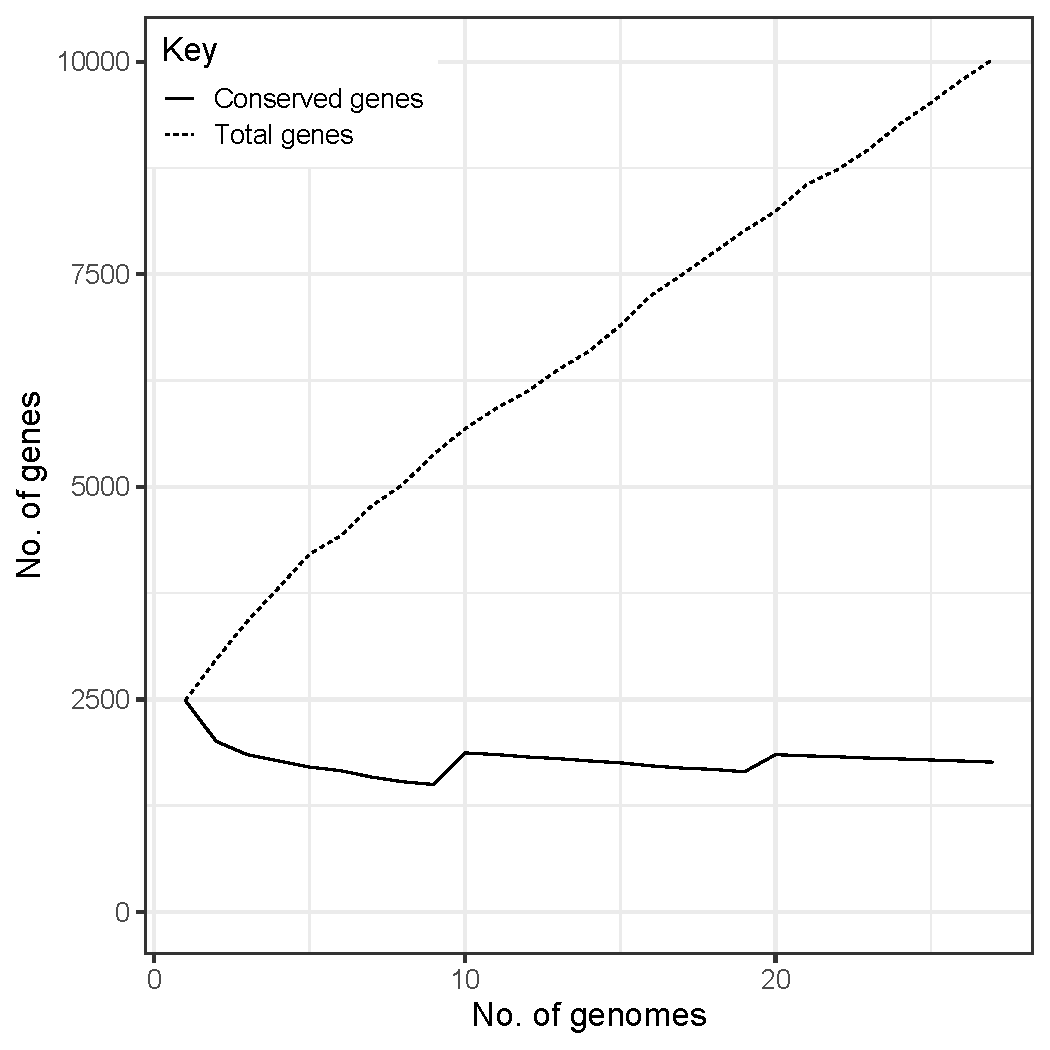
\includegraphics[width=.8\linewidth]{ProjectCMG/images/Rplot1.pdf}
     \caption{Conserved genes and total genes across pangenome}\label{fig:roary1_2}
   \end{minipage}\hfill
   \begin{minipage}{0.48\textwidth}
     \centering
     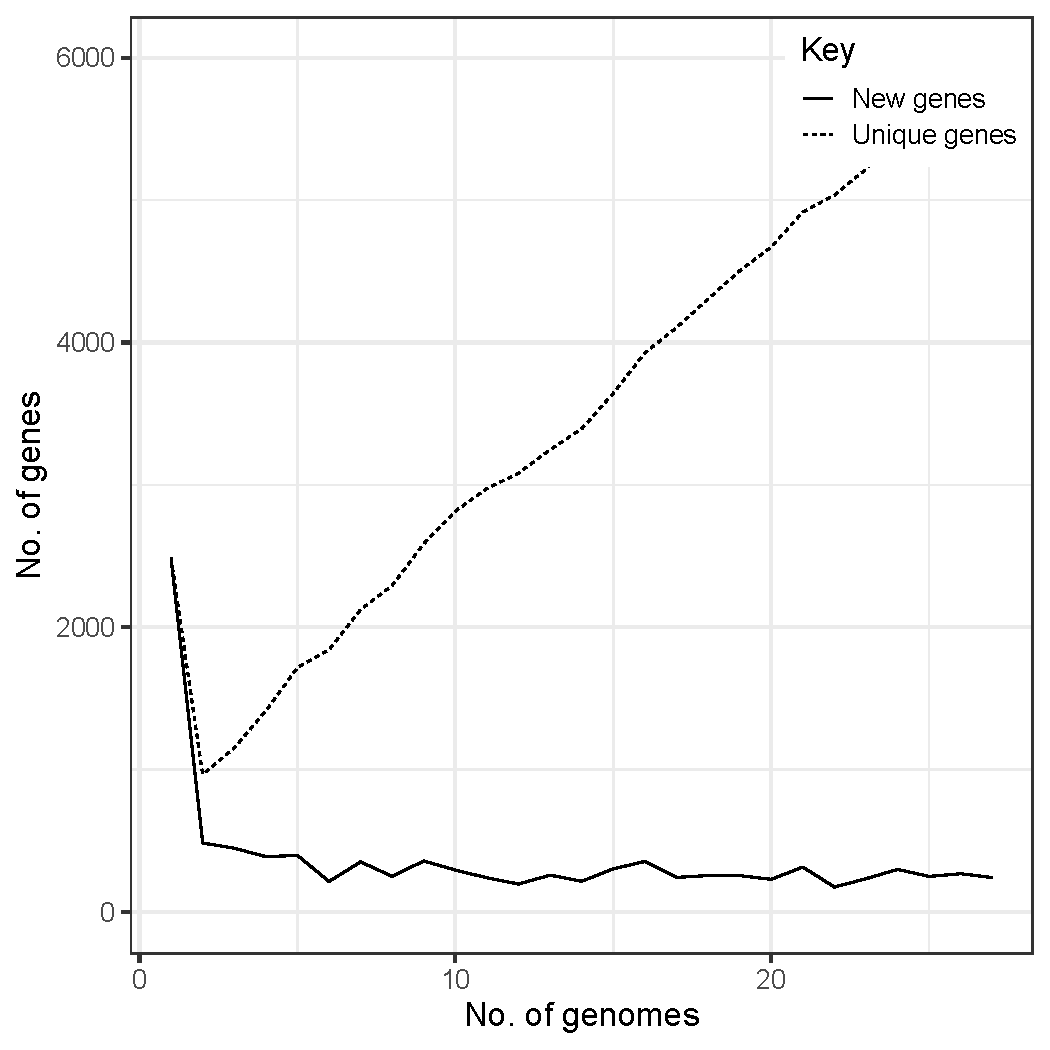
\includegraphics[width=.8\linewidth]{ProjectCMG/images/Rplot2.pdf}
     \caption{New genes and unique genes across pangenome}\label{fig:roary1_3}
   \end{minipage}
\end{figure}

\begin{figure}
    \centering
     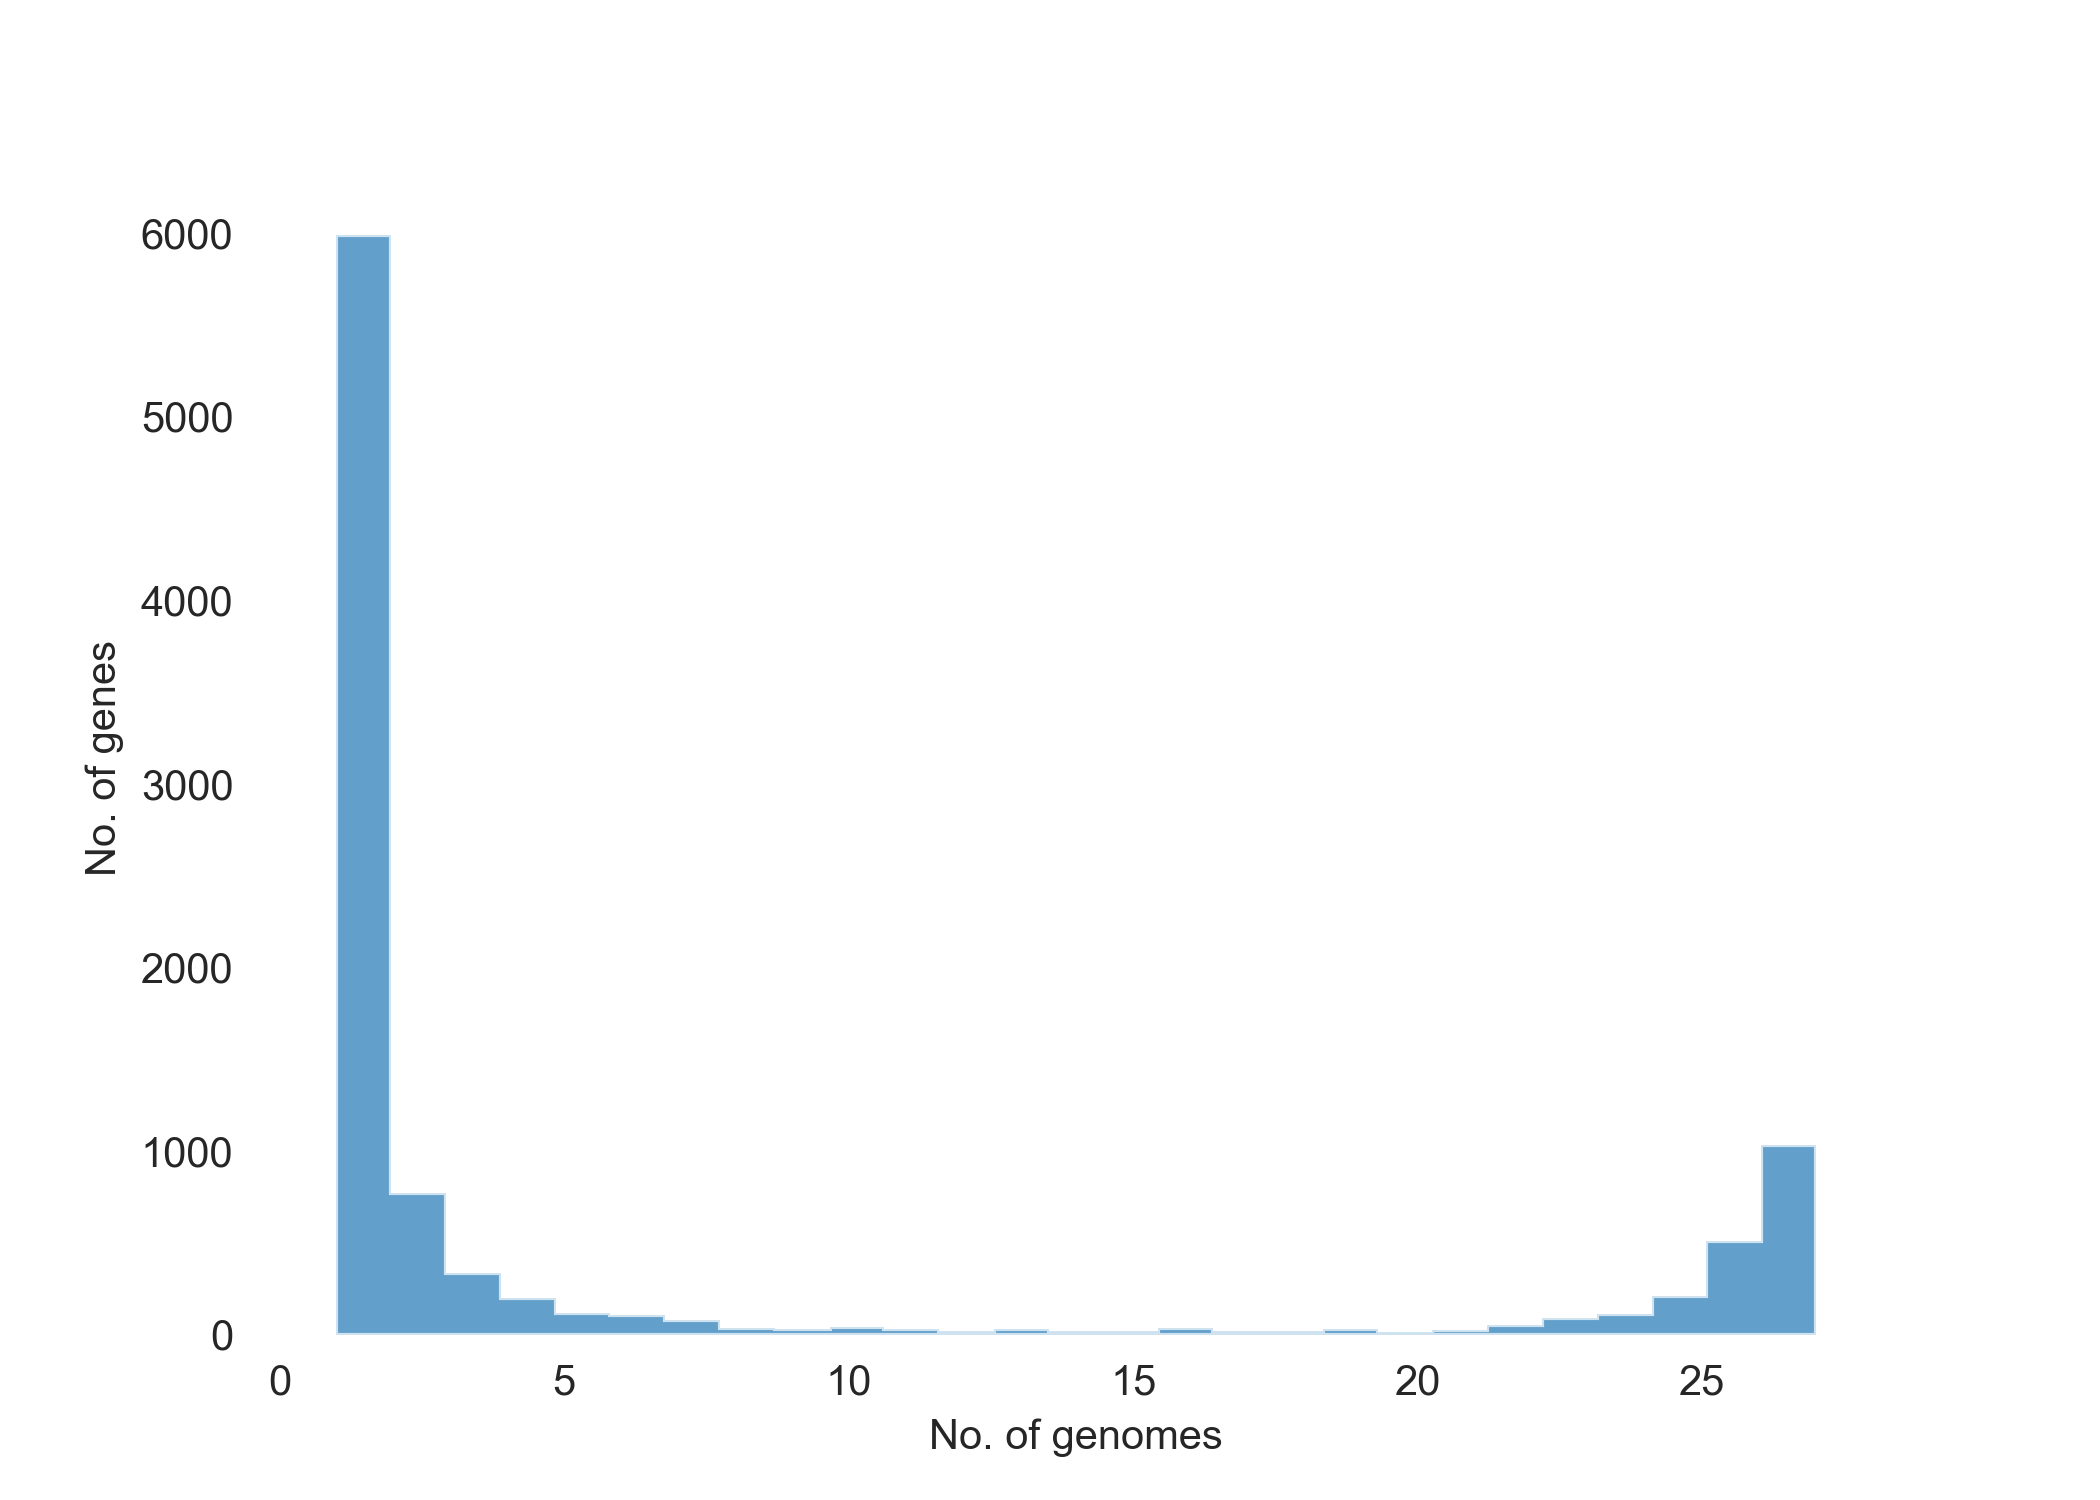
\includegraphics[width=.7\linewidth]{ProjectCMG/images/pangenome_frequency.png}
     \caption{Frequency of genes across pangenome }\label{fig:roary1_freq}
\end{figure}

We observed a small proportion of core genes present in the 27 genomes/strains whereas a large proportion of genes is specific to single or few genomes. Genes specific to few genomes could be newly acquired genes or unique genes of the given genome (Figure \ref{fig:roary1_freq}). We obtained a total of 10028 genes, wherein 1036 were core genes, 513 soft-core genes, 1180 shell genes and 7299 were cloud genes (Figure \ref{fig:roary1_pie}). Through the heatmap we obtained the presence and absence of 10028 genes. We found that only approx. one-tenth of total genes are present in all the strains, i.e. are core genes. Majority of genes are not present in all the strains. This could indicate that this pangenome has lesser core genes, and many accessory genes are strain-specific (Figure \ref{fig:roary1_matrix}). 

\begin{figure}
    \centering
     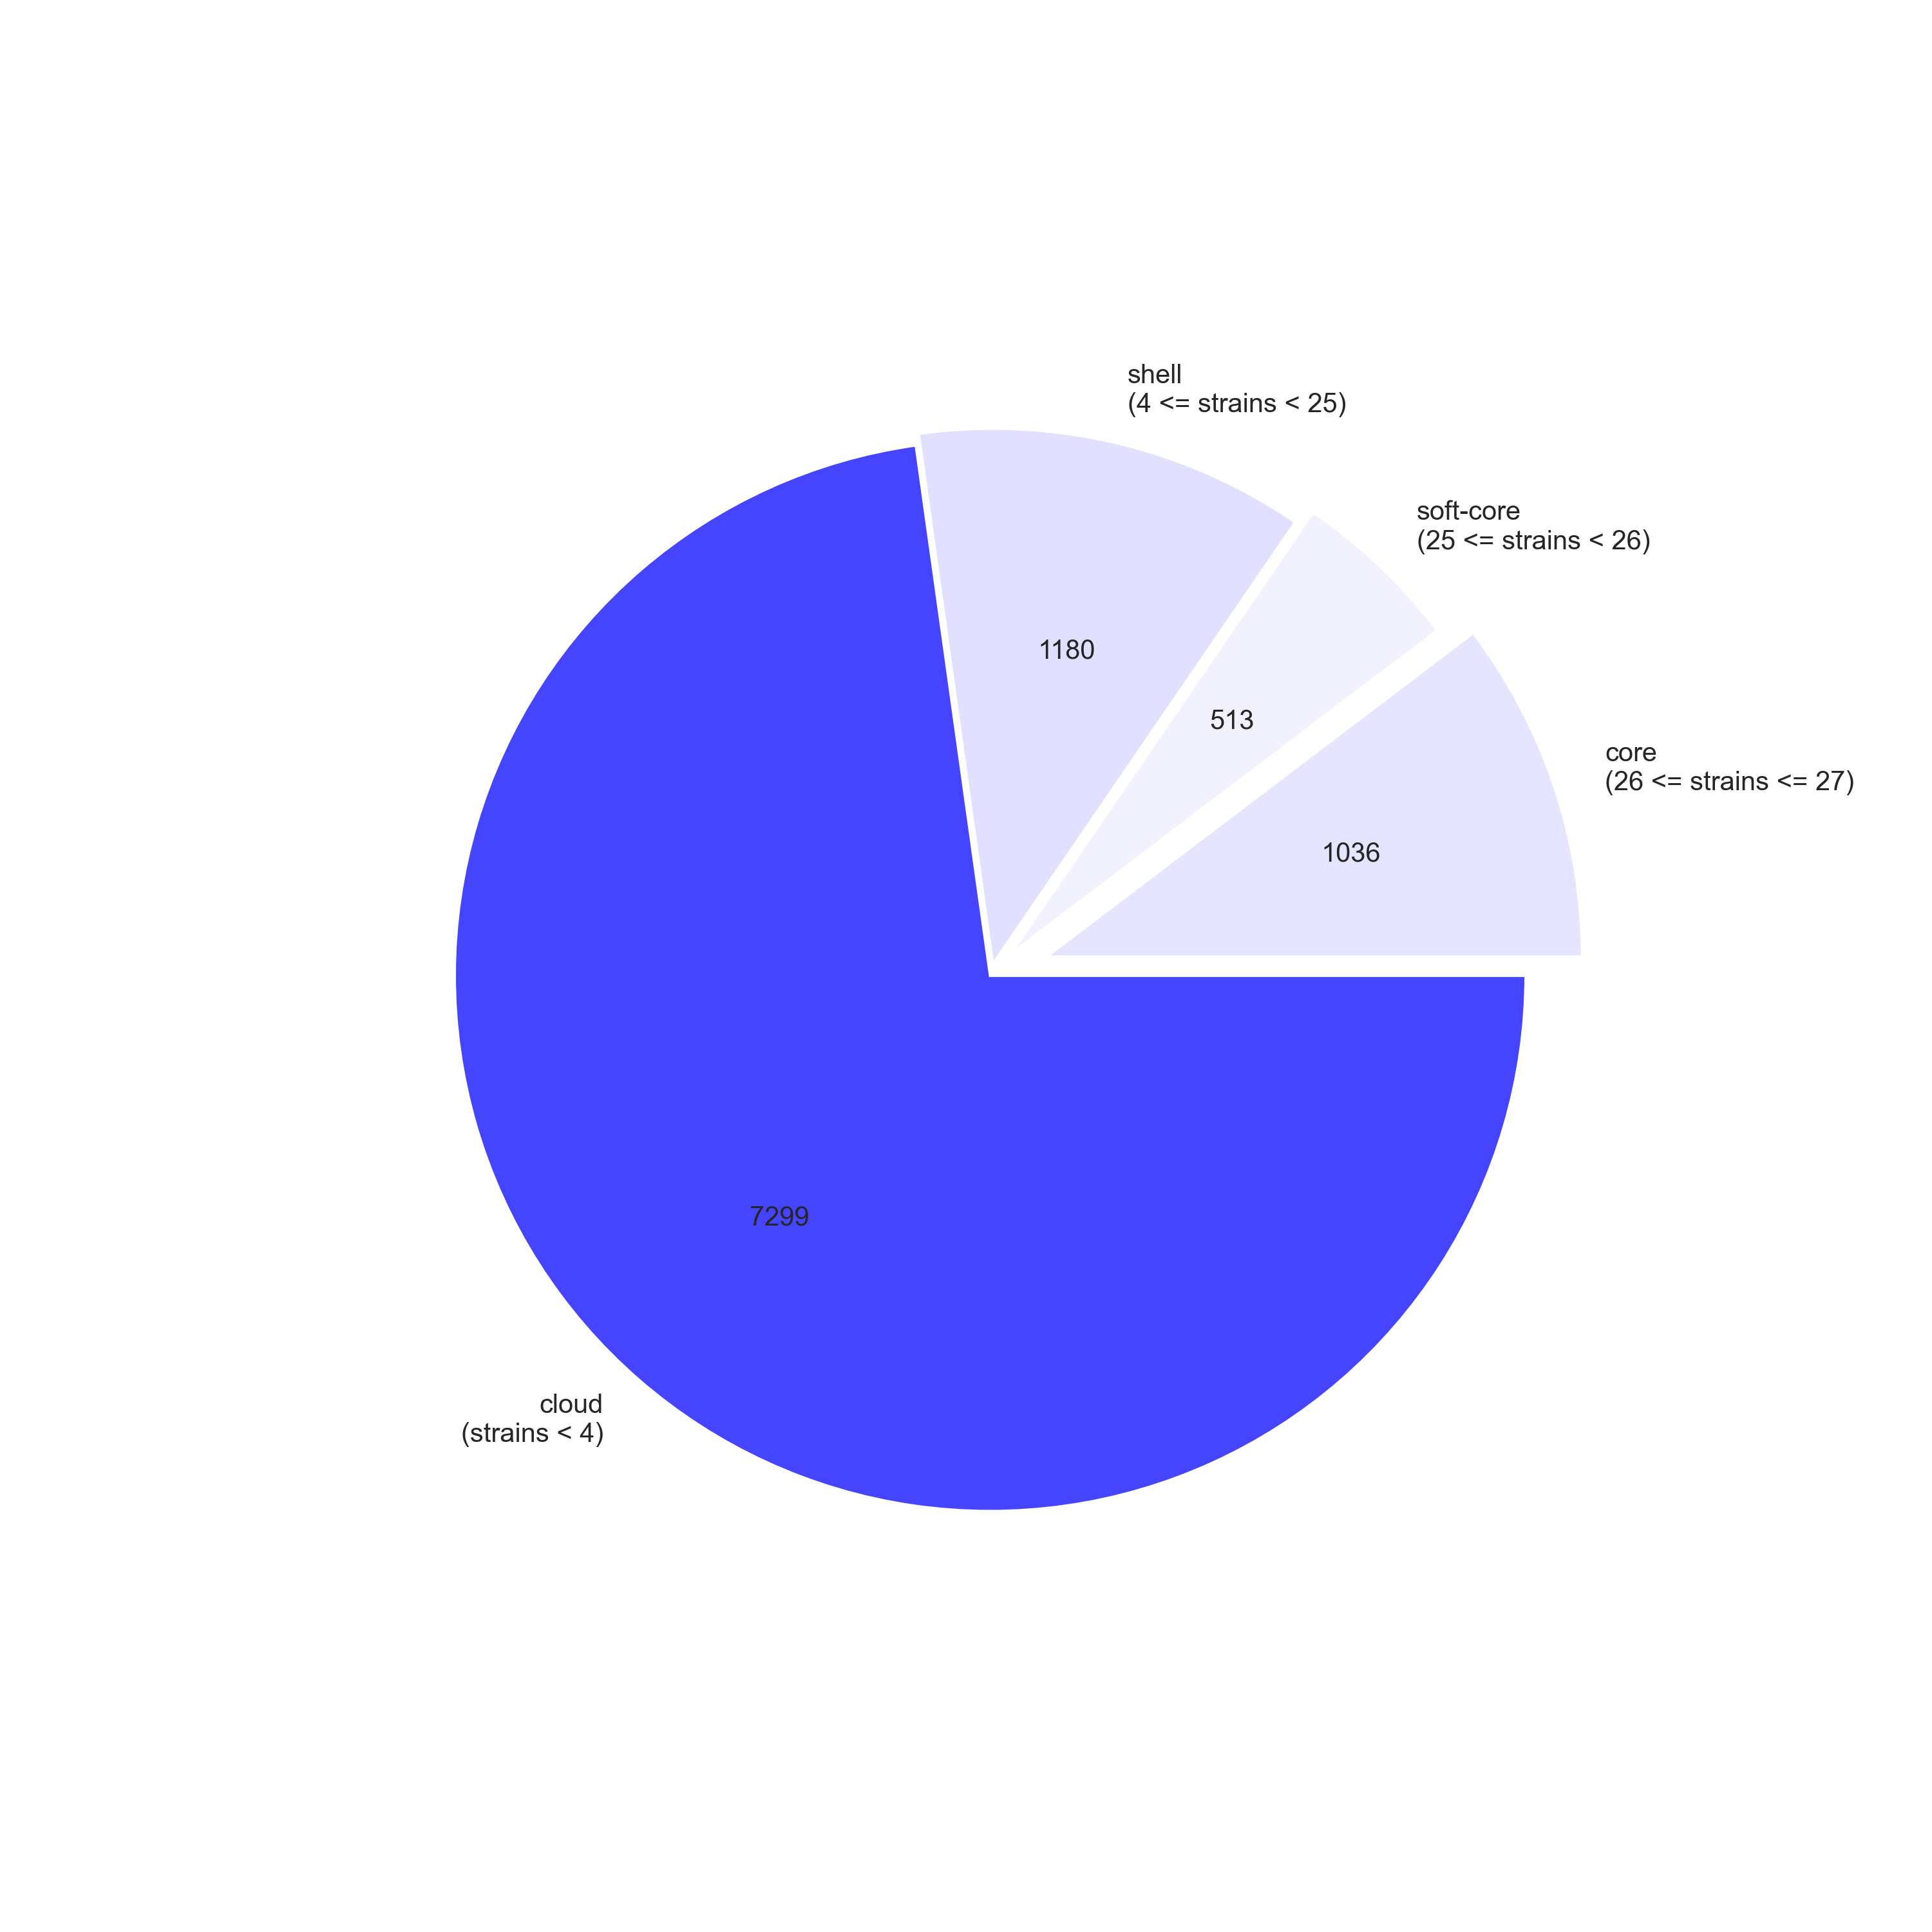
\includegraphics[width=.9\linewidth]{ProjectCMG/images/pangenome_pie.png}
     \caption{Pangenome genes composition: cloud (7299), shell (1180), soft-core (513) and core (1036) genes}\label{fig:roary1_pie}
\end{figure}

\begin{figure}[h!]
    \centering
    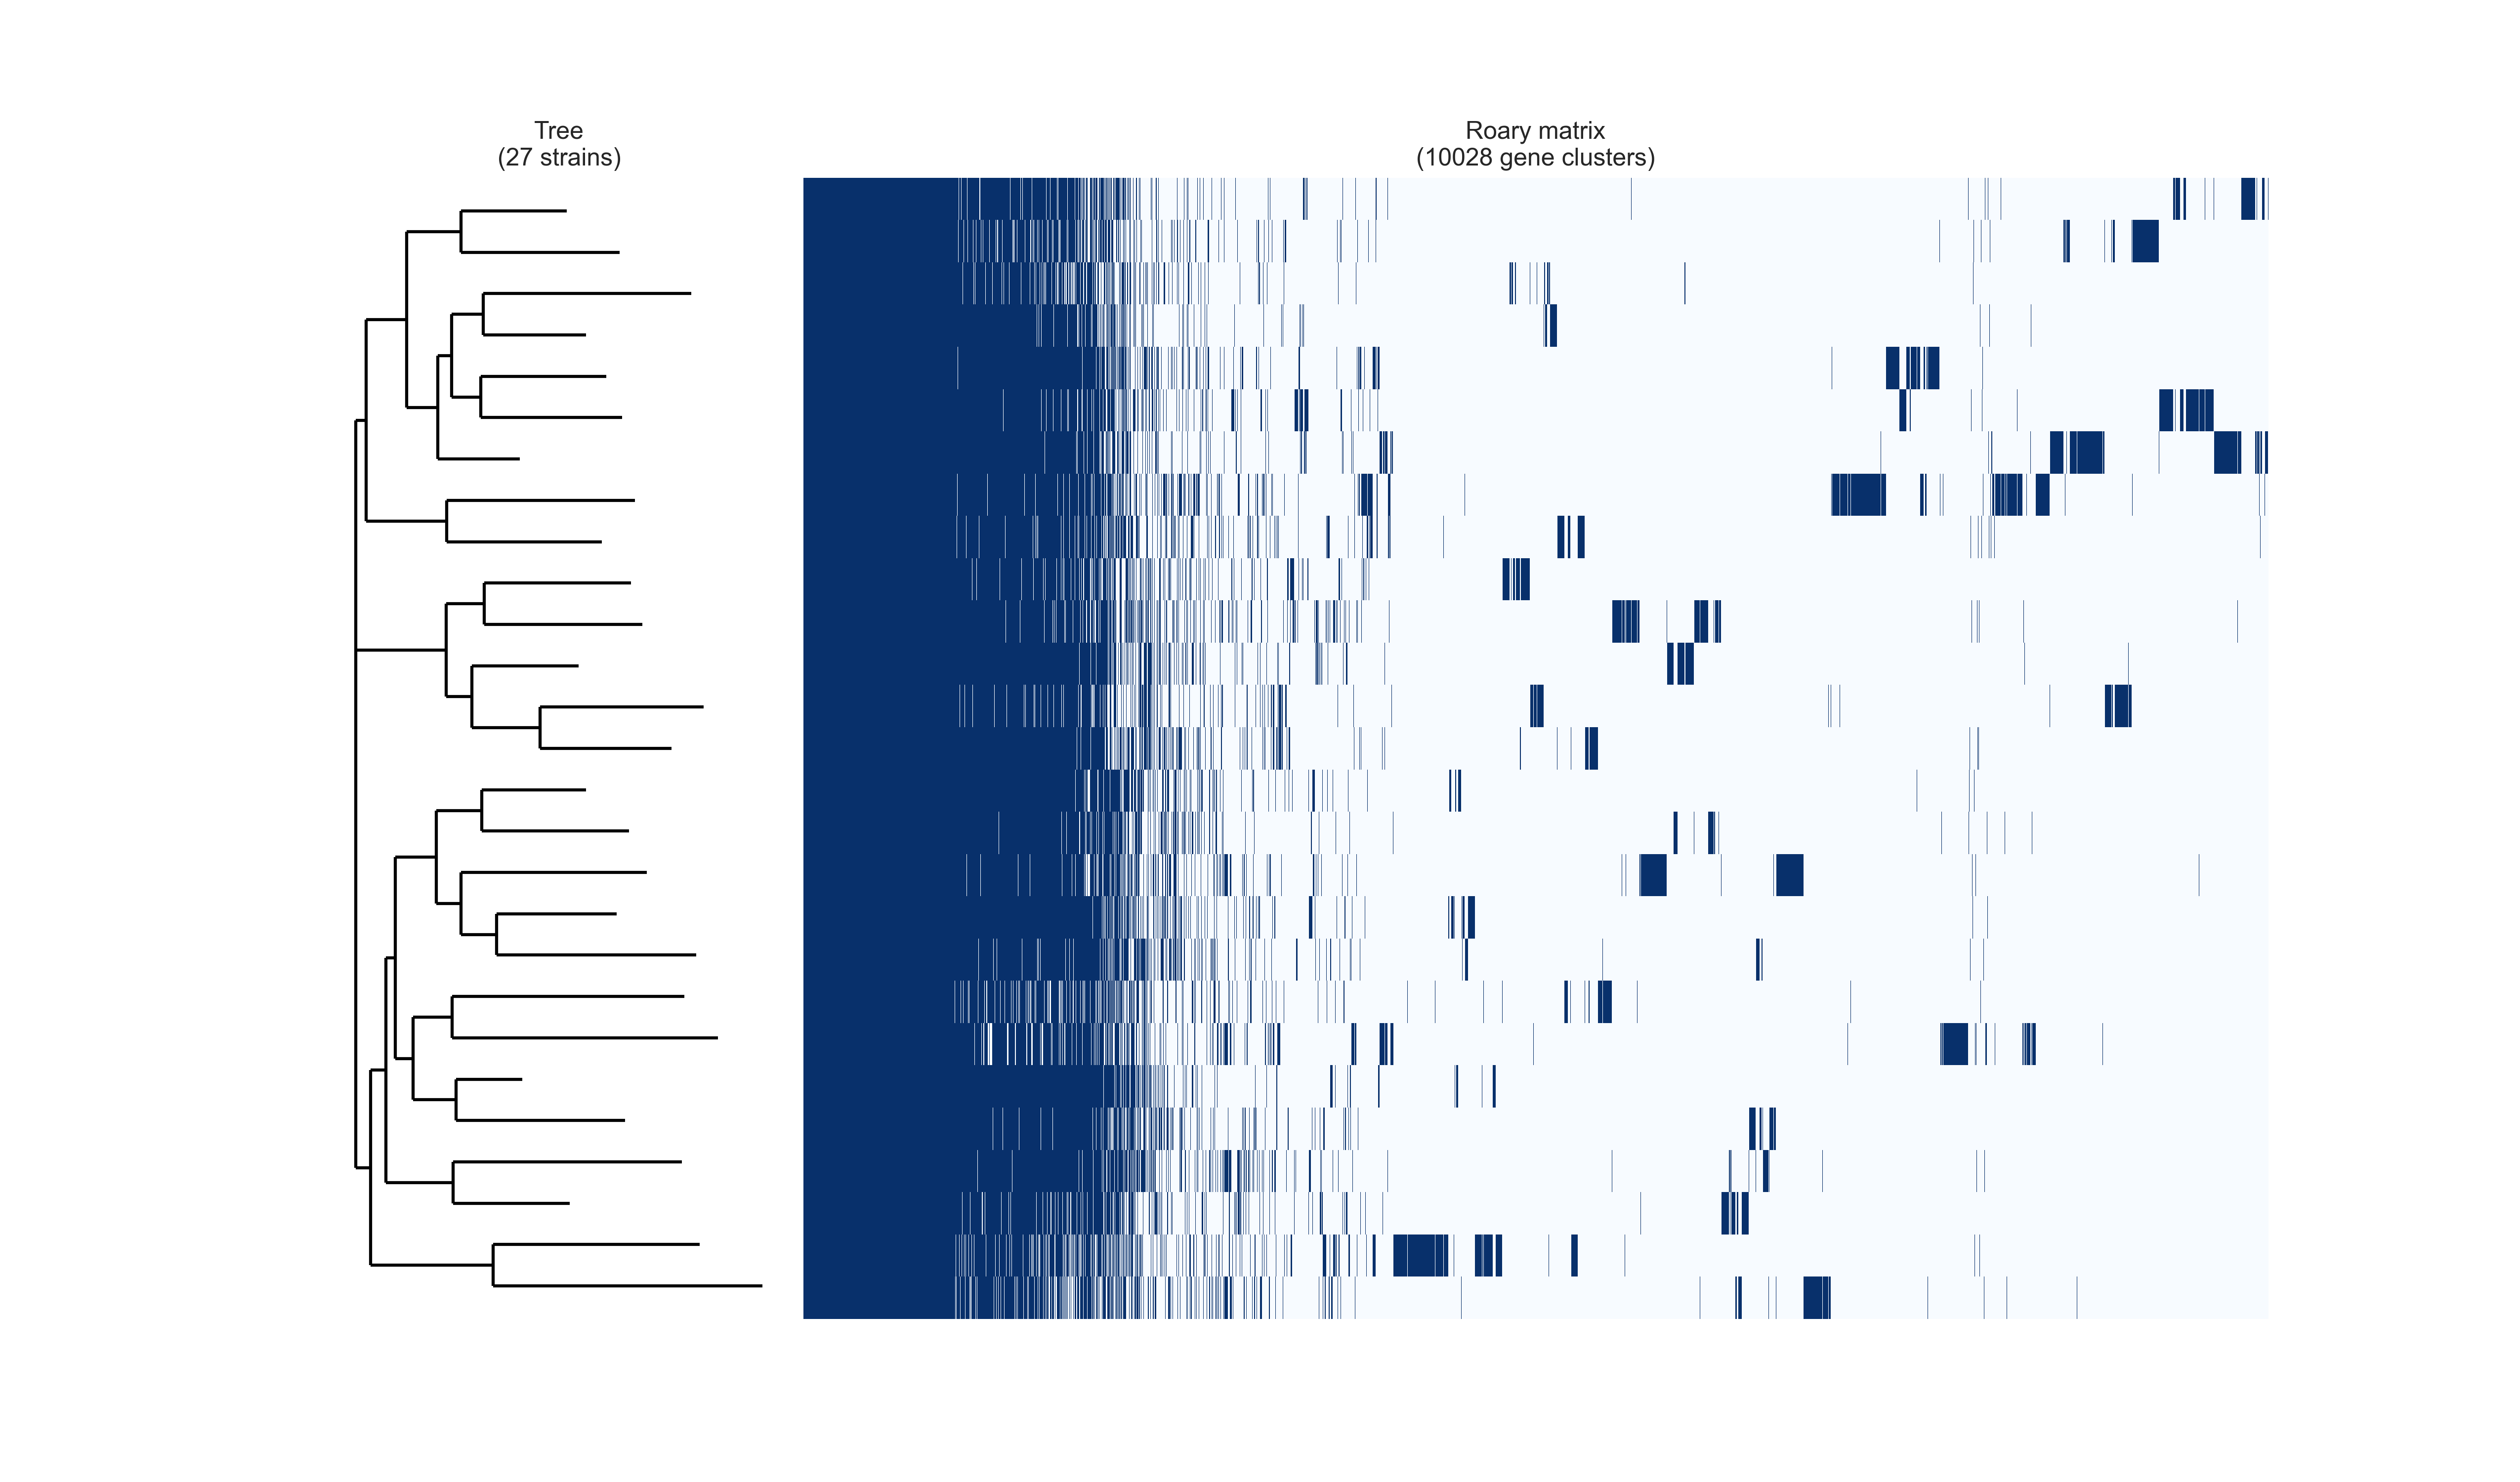
\includegraphics[width=1.1\linewidth]{ProjectCMG/images/pangenome_matrix.png}
    \caption{Heatmap of pangenome. Dark blue represents gene presence; light blue represents gene absence.The x-axis represents 10028 genes clusters and y-axis represents 27 strains in dendrogram. The gene clusters at left in dark blue depicts core genes.}
    \label{fig:roary1_matrix}
\end{figure}

\subsection{Roary: using alignment with MAFFT and PRANK }

After the core genes alignment, the number of Blastp hits under different percentage identity (Figure \ref{fig:roary2_1}), increase in total and unique genes, decrease in conserved genes and new genes per total number of genomes (Figures \ref{fig:roary2_2},\ref{fig:roary2_3}), frequency of genes across pangenome (Figure \ref{fig:roary2_freq}) showed trend similar to previous run of Roary (Figures \ref{fig:roary1_1},\ref{fig:roary1_2},\ref{fig:roary1_3},\ref{fig:roary1_freq}). However, in the second run of Roary, a total 10020 genes with 1035 core genes, 513 soft-core genes, 1181 shell genes and 7291 cloud genes (Figure \ref{fig:roary2_pie}) were found and the presence/absence of genes (Figure \ref{fig:roary2_matrix}) varied as well (Figures \ref{fig:roary1_pie}, \ref{fig:roary1_matrix}).
\newpage
This is due to differences in the working of alignment software used by Roary, thus indicating Blastp implementation is less sensitive than the PRANK and MAFFT in finding core and accessory genes.\\

\subsection{Phylogenetic structure}
From the phylogeny of aligned core genes in the pangenome, we observed three superclades with strains from individuals from different geographical locations clustered together (Figures \ref{fig:Fast_Tree_Core_alignment},\ref{Table:SGB_metadata}). The topmost superclade had 
ViscontiA\_2019SID129237 (Great Britain, GBR), LiJ\_2014V1.UC22-1 (Spain) and XieH\_2016YSZC12003\_35705 (GBR) clustered. QinN\_2014LD-41 (China; HBV+HDV+Cirrhosis), QinJ\_2012T2D-014 (China; T2D), ShaoY\_2019a504a8ac-7ae6-11e9-a106-68b59976a384 (GBR), ShaoY\_2019-\_\\ SID815390bc-7ae6-11e9-a106-68b59976a384 (GBR), YuJ\_2015SZAXPI015233-19 (CHN), YuJ\_2015SZAXPI015252-43 (CHN), YuJ\_2015SZAXPI003424-12 (CHN), PasolliE\_2018\ \\ \_Madagascar      A14\_01\_1FE\_CM\_MDG\_14011 (Madagascar) and GCA900540255 (isolate), NayfachS\_2020\_GEM\_3300029556 (unknown), CM\_Guinea GUI\_80104 (Guinea) clustered together. The other strains clustered in the bottom-most superclade were 1 from Italy (CM\_Neuroblastoma\_NB\_CTR79), 3 from GBR (ShaoY\_2019 b3923042-7ae6-11e9-a106-68b59976a384, ShaoY\_2019 afafe9a6-7ae6-11e9-a106-68b59976a384, \\ ShaoY\_2019cc7b0cfa-7ae6-11e9-a106-68b59976a384) and rest 8 from Guinea (CM guinea2 strains). This indicates that the core genes from all strains express uniformly in guts of different individuals from different geographical locations and might indicate that they  undergo balanced selection. The gut microbial strains of individuals with comorbidities or single disease clustered freely with those of healthy individuals and \textit{Clostridium} isolate, hence, suggest little indication of these strains in causation of these diseases. However, we need to re-affirm this fact by examining more diseased individuals. The gut microbiome of T2D and CRC patients has elevated diversity of species from phylum Firmicutes, class Clostridia whereas liver cirrhosis patients have similar overall microbiome representation as in healthy ones \cite{Qin2012, Qin2014, Nayfach_2019, Armour2019}. Further research is needed to understand the \\ \textit{Clostridium}-disease pathogenic associations.\\

From the phylogeny of accessory genes in the pangenome, based on genes' presence/absence, we detected some patterns of microbiome diversity among individuals from different geographical locations (Figures \ref{fig:Fast_Tree_Presence_Absence},\ref{Table:SGB_metadata}). Four samples from- China (2; 1 unknown health condition and 1 with CRC), Madagascar (1; healthy), Guinea (1; healthy) clustered with the isolate GCA\_900540255 in the first superclade. We noticed that rest 8 samples from Guinea (healthy and non-westernised (NW) except CM\_guinea\_ GUI0080302- westernized) clustered together along with NayfachS\_2019 sample unlike their clustering of their core genes (Figures \ref{fig:Fast_Tree_Core_alignment}, \ref{Table:SGB_metadata}). The remaining samples from- GBR (5; healthy), Italy (1; healthy), Spain (1; healthy), China (4; 2 diseased and 2 unknown health condition), all from westernized populations, clustered together. This confers that the geographical location and lifestyle conditions govern the fixation/loss of accessory genes  of the \textit{Clostridium} spp. in the human gut of individuals from a given geo-location. We recognised that the core and accessory genes of the \textit{Clostridium} isolate is closer to samples from Guinea (NW), Madagascar (NW) and China (westernized)  than to GBR, Spain or Italy. 

\begin{figure}
    \centering
       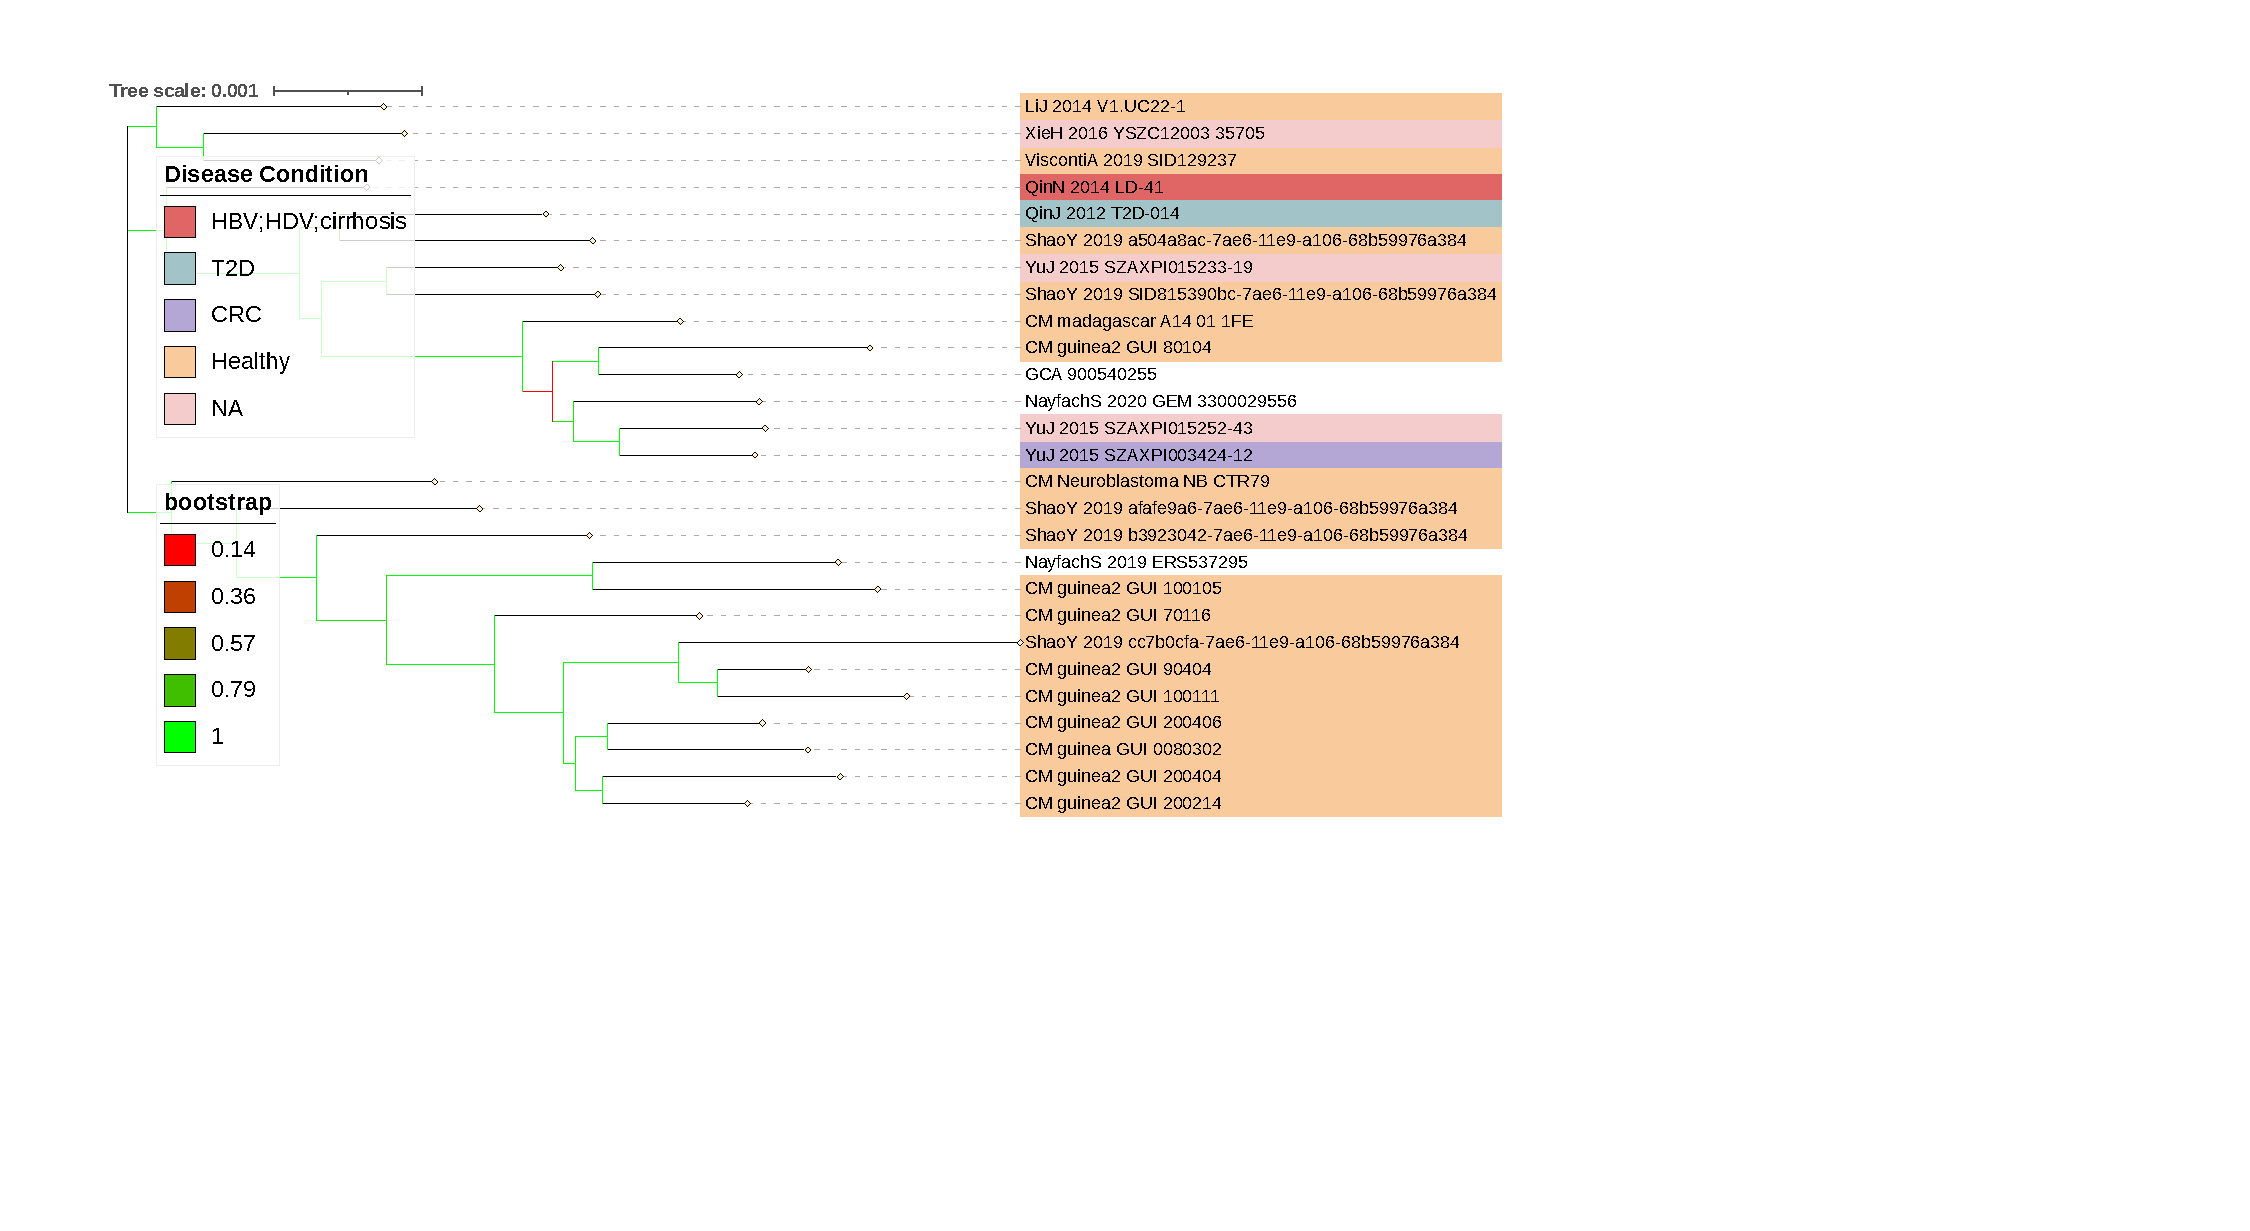
\includegraphics[width=1.6\linewidth]{ProjectCMG/images/core_alignment_tree.pdf}
    \caption{Phylogenetic tree through core genes alignment. The gut microbiome MAGs from healthy individuals are indicated in yellow, diseased patient with HBV (Hepatitis-V) + HDV (Hepatitis-D) + Liver cirrhosis in red, T2D (Type 2 Diabetes) in green and CRC (Colorectal Cancer) in purple. The \textit{Clostridium} isolate and NayfachS samples in white and individuals with unknown health condition in pink.}
    \label{fig:Fast_Tree_Core_alignment}
\end{figure}

\begin{figure}
    \centering
       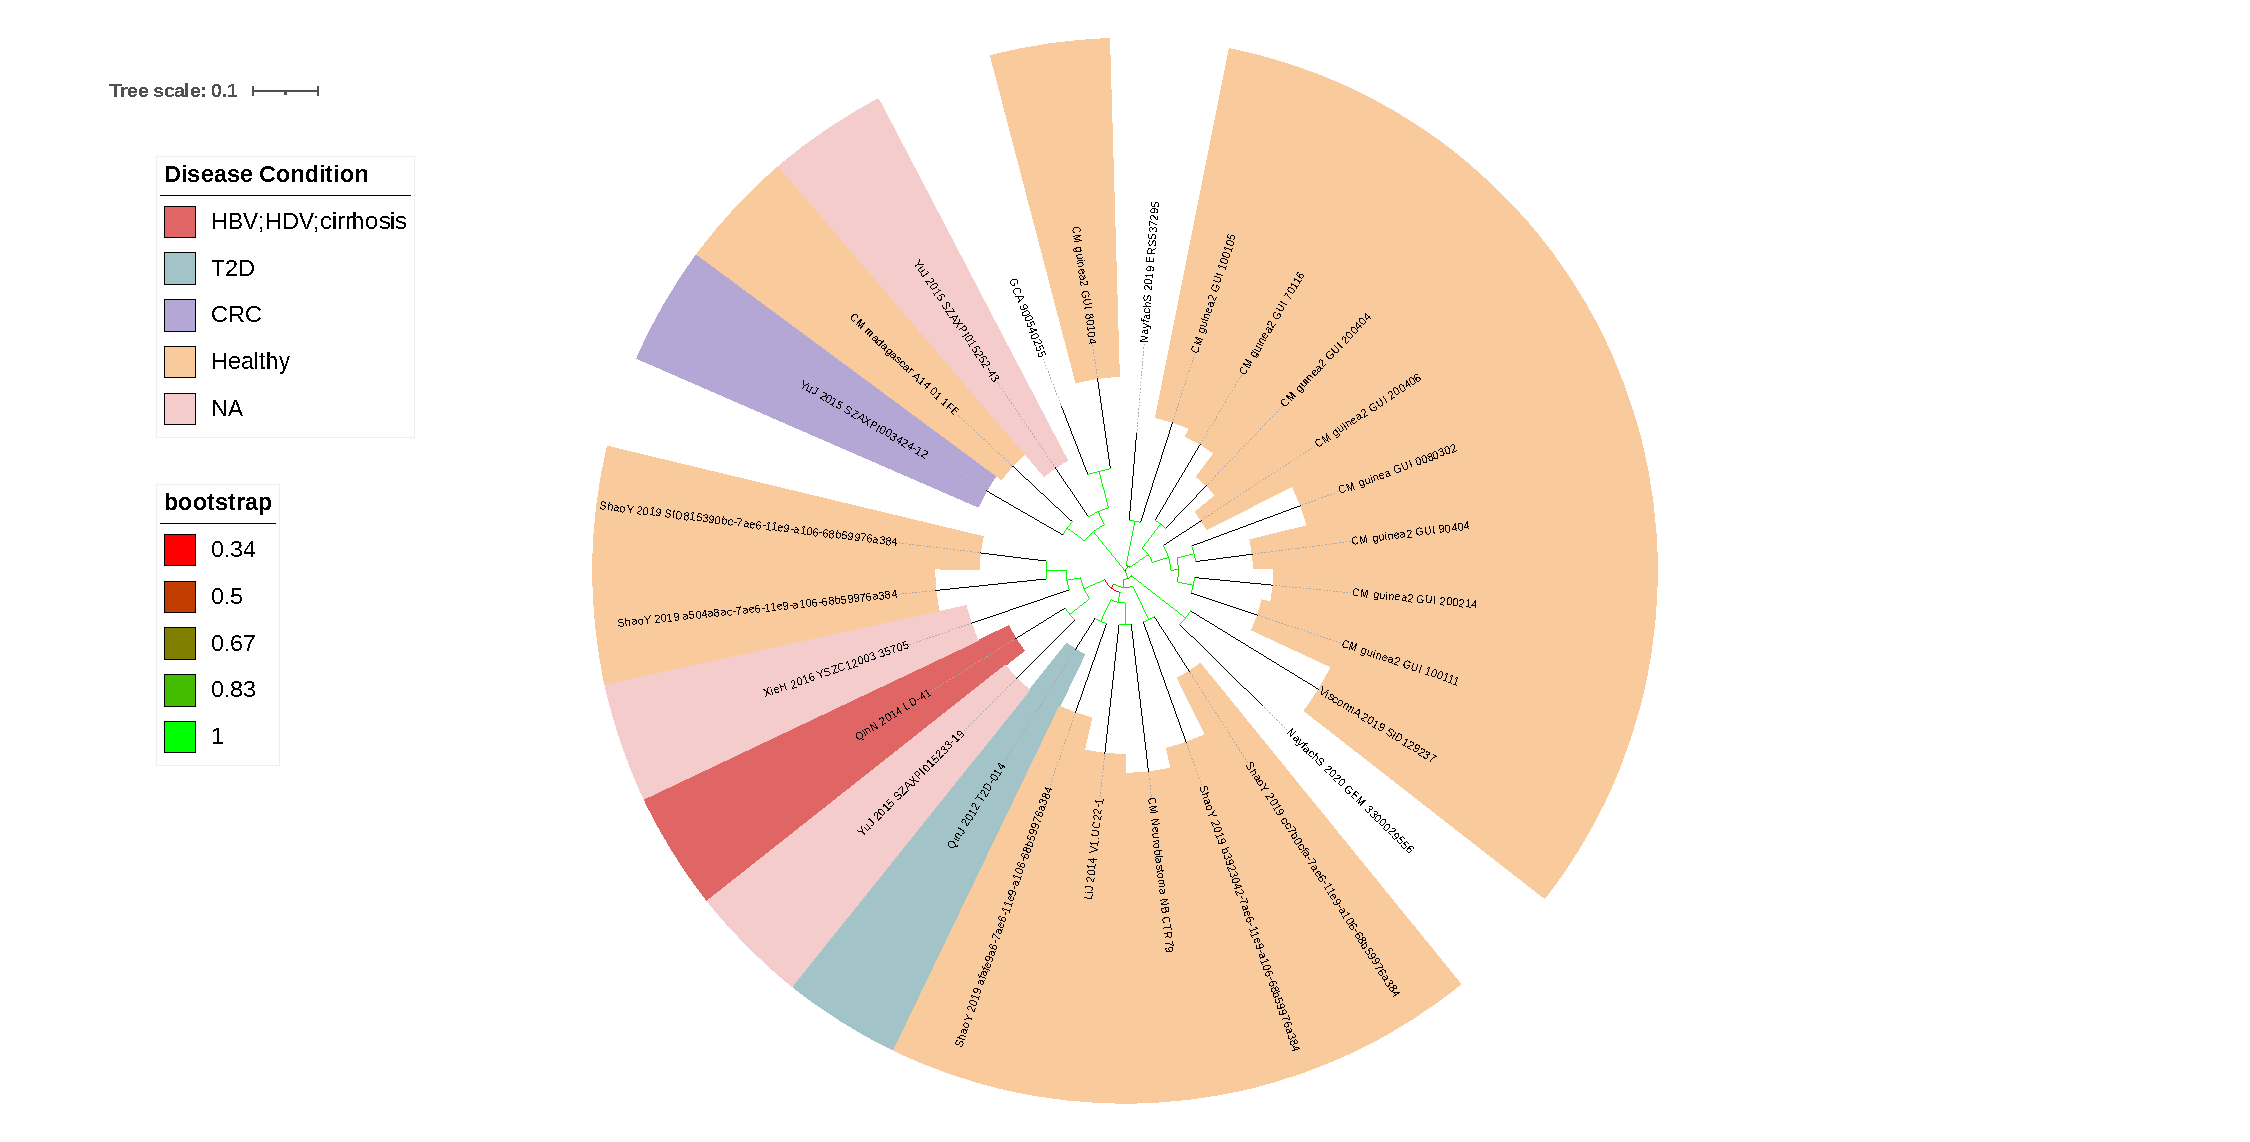
\includegraphics[width=1.4\linewidth]{ProjectCMG/images/first_tree.pdf}
    \caption{Phylogenetic tree of accessory genes indicating their presence/absence. The gut microbiome MAGs from healthy individuals are indicated in yellow, diseased patient with HBV (Hepatitis-V) + HDV (Hepatitis-D) + Liver cirrhosis in red, T2D (Type 2 Diabetes) in green and CRC (Colorectal Cancer) in purple. The \textit{Clostridium} isolate and NayfachS samples in white and individuals with unknown health condition in pink. }
    \label{fig:Fast_Tree_Presence_Absence}
\end{figure}

\subsection{Taxonomic characterisation}
We noticed that all MAGs and the isolate had $<$0.05 as taxonomical distances, which means strong similarities among the different MAGs. We observed that each human gut microbiome represents a different strain of the same species \textit{Clostridium SGB6179}. The phylogenetic richness is typical of Firmicutes, class Clostridia \cite{Forster2019} hence, the phylogenetic tree in our study even corroborates this fact that, Clostridia has open pangenome, possibly due to lateral gene transfer among strains \cite{Qin2012}.\\ 

The MAGs contribute to functional characterisation and taxonomical classification of unfamiliar less copious human gut microbial species and their potential role in pathogenicity and physiology inside host human gut\cite{Jin2022,Almeida2019}. The construction of MAGs from \newline metagenomes databases could diagnose the genetic distinctness and novelty of human gut microbiome among populations worldwide \cite{Nayfach_2019, Asnicar2020} which we witnessed in this study. Such studies can accelerate disease diagnostics and possible cure for human diseases and characterise microbes within the microbiomes which incur diseases non-specifically or specifically as discussed in \cite{Armour2019}. We found that the accessory genes could be population-specific corroborating to recent findings\cite{Almeida2019}. Crucial metabolic pathways and many housekeeping genes-related pathways are driven by core genes (i.e. genes found in more than 90\% of conspecific genomes). Contrarily, accessory genes (i.e. genes found in less than 10\% of conspecific genomes) regulate recombination, replication, comprise mobile genetic elements and  control defense and resistance machinery\cite{Almeida2019}. We found that this uSGB belongs to \textit{Clostridium} spp. and according to some studies\cite{Ferretti2018}, that a single strain colonises adult human gut, it would be meaningful to identify such predominant strains and their level of the pathogenicity among different populations for this uSGB. 

\section{Conclusions}

We studied that different MAGs inside uSGB belong to \textit{Clostridium} spp. We even found several new and unique genes in the pangenome constructed from these MAGs. We found that the pangenome is open in nature, i.e. acquiring new genes gradually. The core genes are roughly conserved among all MAGs despite the samples were obtained from different geographical locations. But, we noticed that the accessory genes are fixing in the various populations and becoming population-specific, inferring that the geography and lifestyle plays a role in such a phenomenon. 


\newpage


%%%%%%%%%%%%%%%%%
% REFERENCES  %
%%%%%%%%%%%%%%%%%

\section{References}
\bibliographystyle{IEEEtran}
\bibliography{biblio}
\newpage

%%%%%%%%%%%%%%%%%%%%
% APPENDIX         %
%%%%%%%%%%%%%%%%%%%%
\section{Appendix}
%subsection{SGB6179 data}
\begin{landscape}
\begin{table}[h]
\begin{center}
%\begin{adjustbox}{width=\textwidth}
\small
    \begin{tabular}{|c|c|c|c|c|c|}
        \hline
        Dataset name & Sample ID &  Number of reads & Number of bases & Minimum read length & Median read length\\
        \hline
        LiJ\_2014 & V1.UC22-1 & 82978692 & 6823277690 & 30 & 86 \\
        QinJ\_2012 & T2D-014 & 52225992 & 4700339280 & 90 & 90\\
        QinN\_2014 & LD-41  & 52250886 & 5225088600 & 100 & 100 \\
        XieH\_2016 & YSZC12003\_35705 & 66991690 & 6564082392 & 30 & 100 \\
        YuJ\_2015 & SZAXPI003424-12 & 58546892 & 5593003062 & 30 & 100\\
        YuJ\_2015 & SZAXPI015233-19 & 72077438 & 7024760687 & 30 & 100\\
        YuJ\_2015 & SZAXPI015252-43 & 44904362 & 4378527165 & 30 & 100\\
        CM\_Guinea & GUI\_0080302 & 37003882 & 3718239745 & 75 & 101 \\
        CM\_Guinea & GUI\_100105 & 49958829 & 7499685933 & 75 & 151 \\
        CM\_Guinea & GUI\_100111 & 46045645 & 6918322696 & 75 & 151 \\
        CM\_Guinea & GUI\_200214 & 48425161 & 7270574229 & 75 & 151 \\
        CM\_Guinea & GUI\_200404  & 61377875 & 9213316332 & 75 & 151\\
        CM\_Guinea & GUI\_200406 & 49968611 & 7507455459 & 75 & 151 \\
        CM\_Guinea & GUI\_70116  & 46373584 & 6970616703 & 75 & 151 \\
        CM\_Guinea & GUI\_80104 & 62630186 & 9407192009 & 75 & 151 \\
        CM\_Guinea & GUI\_90404 & 23708901 & 3556954184 & 75 & 151\\
        CM\_NEUROBLASTOMA & NB\_CTR79 & 54826722 & 8235060533 & 75 & 151\\
        PasolliE\_2018\_Madagascar & A14\_01\_1FE  & 51877496 & 5117619802 & 75 & 101 \\
        ShaoY\_2019 & a504a8ac-7ae6-11e9-a106-68b59976a384 & 13388070 & 1646174990 & NA & 125 \\
        ShaoY\_2019 & cc7b0cfa-7ae6-11e9-a106-68b59976a384 &  16934168 & 2009984998 & NA & 125 \\
        ShaoY\_2019 & b3923042-7ae6-11e9-a106-68b59976a384 & 18601446 & 2235383168 & NA & 125 \\
        ShaoY\_2019 & afafe9a6-7ae6-11e9-a106-68b59976a384 & 16019068 & 1918265711 & NA & 125\\
        ShaoY\_2019 & SID815390bc-7ae6-11e9-a106-68b59976a384 & 19783784 & 2378314506 &	NA & 125\\
        ViscontiA\_2019 & SID129237 & 50085124 & 5839317670 & 75 & 124 \\
        \hline
    \end{tabular}\\
%    \end{adjustbox}
    \caption{SGB6179 metadata: Moreover, in our dataset, we had also a genome coming from known isolated organism, \textit{Clostridium sp.}. This genome is present in our dataset as GCA\_900540255.fna.}
    \label{Table:SGB_metadata}
\end{center}   
\end{table}
\end{landscape}

\begin{landscape}
\begin{table}[h]
\begin{center}
%\begin{adjustbox}{width=\textwidth}
\small
    \begin{tabular}{|c|c|c|c|c|c|c|c|}
        \hline
        Dataset name & Subject ID &  Study conditions & Disease & Age & Gender & Country & Non Westernized \\
        \hline
        LiJ\_2014 & V1.UC22-1 & control & healthy & NA & NA & ESP & no\\
        QinJ\_2012 & T2D-014 &  T2D &  T2D &  63 &  female & CHN & no\\
        QinN\_2014 &  LD-41	& cirrhosis &  HBV;HDV;cirrhosis &  47 &  female & CHN & no\\
        XieH\_2016 &  YSZC12003\_35705 &  control &  NA &  68 &  female & GBR & no\\
        YuJ\_2015 & SZAXPI003424-12 &  CRC &  CRC &  NA &  NA & CHN & no\\
        YuJ\_2015 & SZAXPI015233-19 &  control &  NA &  NA &  NA & CHN & no\\
        YuJ\_2015 & SZAXPI015252-43 &  control &  NA &  NA &  NA & CHN & no\\
        CM\_Guinea &GUI\_0080302 & control & healthy & 24 & female & GUI & no\\
        CM\_Guinea & GUI\_100105 & control & healthy & 6 & female & GUI & yes \\
        CM\_Guinea & GUI\_100111 & control & healthy & 6 & female & GUI & yes\\
        CM\_Guinea & GUI\_200214 & control & healthy & NA & NA  & GUI & yes\\
        CM\_Guinea & GUI\_200404  & control & healthy & 20 & female & GUI & yes\\
        CM\_Guinea & GUI\_200406 & control & healthy & 16 & female  & GUI & yes\\
        CM\_Guinea & GUI\_70116  & control & healthy & 45 & female  & GUI & yes\\
        CM\_Guinea & GUI\_80104 & control & healthy & 8 & male  & GUI & yes\\
        CM\_Guinea & GUI\_90404 & control & healthy & 4 & female & GUI & yes\\
        CM\_NEUROBLASTOMA & NB\_CTR79 & control & healthy & 5.8 & male & ITA & N\\
        PasolliE\_2018\_Madagascar & CM\_MDG\_14011 & control & healthy & 36 & male & MDG & yes\\
        ShaoY\_2019 & B01339 & control & healthy & 0.010958904 & male & GBR & no \\
        ShaoY\_2019 & B02739 & control & healthy & 0.575342466 & male & GBR & no  \\
        ShaoY\_2019 & B01799 & control & healthy & 0.769863014 & female & GBR & no  \\
        ShaoY\_2019 & B01712 & control & healthy & 0.8 & male & GBR & no \\
        ShaoY\_2019 & A01685 & control & healthy & 0 & male & GBR & no \\
        ViscontiA\_2019 & TUK89005992 & control & healthy & 60 & female & GBR & no \\
        \hline
    \end{tabular}\\
%    \end{adjustbox}
    \caption{SGB6179 metadata}
    \label{Table:SGB_metadata2}
\end{center}   
\end{table}
\end{landscape}



\begin{landscape}
\begin{table}[]
    \centering
    \small
    \begin{tabular}{|c|c|c|c|c|}
        \hline
        Bin & Sample & Completeness & Redundancy & SGB \\
        \hline
        CM\_guinea2\_\_GUI\_100105\_\_bin.75 & GUI\_100105 & 94.35 & 2.67 & SGB6179 \\
        CM\_guinea2\_\_GUI\_100111\_\_bin.34 & GUI\_100111 & 95.97 & 0.81 & SGB6179 \\
        CM\_guinea2\_\_GUI\_200214\_\_bin.86 & GUI\_200214 & 95.97 & 1.45 & SGB6179 \\
        CM\_guinea2\_\_GUI\_200404\_\_bin.54 & GUI\_200404 & 92.99 & 3.02 & SGB6179 \\
        CM\_guinea2\_\_GUI\_200406\_\_bin.2 & GUI\_200406 & 95.97 & 1.05 & SGB6179 \\
        CM\_guinea2\_\_GUI\_70116\_\_bin.90 & GUI\_70116 & 92.79 & 1.33 & SGB6179 \\
        CM\_guinea2\_\_GUI\_80104\_\_bin.57 & GUI\_80104 & 95.65 & 4.87 & SGB6179 \\
        CM\_guinea2\_\_GUI\_90404\_\_bin.43 & GUI\_90404 & 95.71 & 3.92 & SGB6179 \\
        CM\_guinea\_\_GUI\_0080302\_\_bin.8 & GUI\_0080302 & 92.1 & 1.37 & SGB6179 \\
        CM\_madagascar\_\_A14\_01\_1FE\_\_bin.13 & A14\_01\_1FE & 95.96774194 & 0.161290323 & SGB6179 \\
        CM\_Neuroblastoma\_\_NB\_CTR79\_\_bin.26 & NB\_CTR79 & 93.86 & 3.5 & SGB6179 \\
        GCA\_900540255 & SAMEA4890906 & 96.77 & 0 & SGB6179 \\
        LiJ\_2014\_\_V1.UC22-1\_\_bin.24 & V1.UC22-1 & 91.46505376 & 2.459677419 & SGB6179 \\
        NayfachS\_2019\_\_ERS537295\_\_bin.57 & ERS537295 & 95.16 & 0 & SGB6179 \\
        NayfachS\_2020\_\_GEM\_3300029556\_\_bin.6 & GEM\_3300029556 & 92.34 & 4.34 & SGB6179 \\
        QinJ\_2012\_\_T2D-014\_\_bin.33 & T2D-014 & 96.77419355 & 0 & SGB6179 \\
        QinN\_2014\_\_LD-41\_\_bin.25 & LD-41 & 94.40092166 & 0.089605735 & SGB6179 \\
        ShaoY\_2019\_\_a504a8ac-7ae6-11e9-a106-68b59976a384\_\_bin.8 & a504a8ac-7ae6-11e9-a106-68b59976a384 & 95.57 & 0.43 & SGB6179 \\
        ShaoY\_2019\_\_afafe9a6-7ae6-11e9-a106-68b59976a384\_\_bin.6 & afafe9a6-7ae6-11e9-a106-68b59976a384 & 94.35 & 0.81 & SGB6179 \\
        ShaoY\_2019\_\_b3923042-7ae6-11e9-a106-68b59976a384\_\_bin.23 & b3923042-7ae6-11e9-a106-68b59976a384 & 95.16 & 1.47 & SGB6179 \\
        ShaoY\_2019\_\_cc7b0cfa-7ae6-11e9-a106-68b59976a384\_\_bin.21 & cc7b0cfa-7ae6-11e9-a106-68b59976a384 & 95.16 & 0.16 & SGB6179 \\
        ShaoY\_2019\_\_SID815390bc-7ae6-11e9-a106-68b59976a384\_\_bin.19 & SID815390bc-7ae6-11e9-a106-68b59976a384 & 95.97 & 0.16 & SGB6179 \\
        ViscontiA\_2019\_\_SID129237\_\_bin.45 & SID129237 & 91.29 & 0 & SGB6179 \\
        XieH\_2016\_\_YSZC12003\_35705\_\_bin.27 & YSZC12003\_35705 & 95.11776754 & 1.500896057 & SGB6179 \\
        YuJ\_2015\_\_SZAXPI003424-12\_\_bin.14 & SZAXPI003424-12 & 95.88709677 & 2.777777778 & SGB6179 \\
        YuJ\_2015\_\_SZAXPI015233-19\_\_bin.67 & SZAXPI015233-19 & 96.77419355 & 0.403225806 & SGB6179 \\
        YuJ\_2015\_\_SZAXPI015252-43\_\_bin.58 & SZAXPI015252-43 & 96.77419355 & 1.792114695 & SGB6179\\
         \hline
    \end{tabular}
    \caption{SGB6179 bin data}
    \label{Table:SGB_bin_data}
\end{table}
\end{landscape}

%\newpage    

%\subsection{PROKKA Outputs}
\begin{landscape}
\begin{table}[h!]
\begin{center}
\small
    \begin{tabular}{|c|c|c|c|c|}
        \hline
        Samples & Number of contigs & CDS counts & Hypothetical proteins & Known proteins \\
        \hline \hline
        CM\_Neuroblastoma\_\_NB\_CTR79\_\_bin.26 & 449 & 2619 & 1231 & 1458\\
        %\hline
        CM\_guinea2\_\_GUI\_100105\_\_bin.75 & 233 & 3192 & 1718 & 1549 \\
        %\hline
        CM\_guinea2\_\_GUI\_100111\_\_bin.34 & 109 & 2688 & 1238 & 1540\\
        %\hline
        CM\_guinea2\_\_GUI\_200214\_\_bin.86 & 282 & 2765 & 1313 & 1525\\
        %\hline
        CM\_guinea2\_\_GUI\_200404\_\_bin.54 & 261 & 2367 & 1027 & 1388\\
        %\hline
        CM\_guinea2\_\_GUI\_200406\_\_bin.2 & 223 & 2900 & 1401 & 1589\\
        %\hline
        CM\_guinea2\_\_GUI\_70116\_\_bin.90 & 339 & 2307 & 1023 & 1360\\
        %\hline
        CM\_guinea2\_\_GUI\_80104\_\_bin.57 & 306 & 2583 & 1142 & 1516\\
        %\hline
        CM\_guinea2\_\_GUI\_90404\_\_bin.43 & 145 & 2244 & 901 & 1412\\
        %\hline
        CM\_guinea\_\_GUI\_0080302\_\_bin.8 & 261 & 2170 & 844 & 1380\\
        %\hline
        CM\_madagascar\_\_A14\_01\_1FE\_\_bin.13 & 261 & 2536 & 1124 & 1447\\
        %\hline
        GCA\_900540255 & 79 & 2568 & 1138 & 1465 \\
        %\hline
        LiJ\_2014\_\_V1.UC22-1\_\_bin.24 & 337 & 2394 & 1036 & 1383\\
        %\hline
        NayfachS\_2019\_\_ERS537295\_\_bin.57 & 150 & 2522 & 1110 & 1467\\
        %\hline
        NayfachS\_2020\_\_GEM\_3300029556\_\_bin.6 & 282 & 2862 & 1334 & 1594 \\
        %\hline
        QinJ\_2012\_\_T2D-014\_\_bin.33 & 72 & 2467 & 1032 & 1513\\
        %\hline
        QinN\_2014\_\_LD-41\_\_bin.25 & 90 & 2471 & 1062 & 1473\\
        %\hline
        ShaoY\_2019\_\_SID815390bc-7ae6-11e9-a106-68b59976a384\_\_bin.19 & 86 & 2570 & 1152 & 1487\\
        %\hline
        ShaoY\_2019\_\_a504a8ac-7ae6-11e9-a106-68b59976a384\_\_bin.8 & 173 & 2531 & 1113 & 1492\\
        %\hline
        ShaoY\_2019\_\_afafe9a6-7ae6-11e9-a106-68b59976a384\_\_bin.6 & 100 & 2565 & 1139 & 1499\\
        %\hline
        ShaoY\_2019\_\_b3923042-7ae6-11e9-a106-68b59976a384\_\_bin.23 & 154 & 2632 & 1176 & 1530\\
        %\hline
        ShaoY\_2019\_\_cc7b0cfa-7ae6-11e9-a106-68b59976a384\_\_bin.21  & 71 & 2495 & 1101 & 1475\\
        %\hline
        ViscontiA\_2019\_\_SID129237\_\_bin.45 & 446 & 2438 & 1058 & 1431\\
        %\hline
        XieH\_2016\_\_YSZC12003\_35705\_\_bin.27 & 232 & 2780 & 1312 & 1537\\
        %\hline
        YuJ\_2015\_\_SZAXPI003424-12\_\_bin.14 & 217 & 2739 & 1207 & 1577\\
        %\hline
        YuJ\_2015\_\_SZAXPI015233-19\_\_bin.67 & 208 & 2446 & 1027 & 1454\\
        %\hline
        YuJ\_2015\_\_SZAXPI015252-43\_\_bin.58 & 112 & 2592 & 1125 & 1523\\
        \hline
    \end{tabular}\\
    \caption{Number of contigs, CDS counts, Hypothetical proteins counts and known proteins counts per sample}
    \label{Table:prokka}
\end{center}   
\end{table}
\end{landscape}

\newpage
%\subsection{Contigs versus Completeness and Redundancy}
\begin{figure}[!htb]
   %\begin{minipage}{0.6\textwidth}
     \centering
     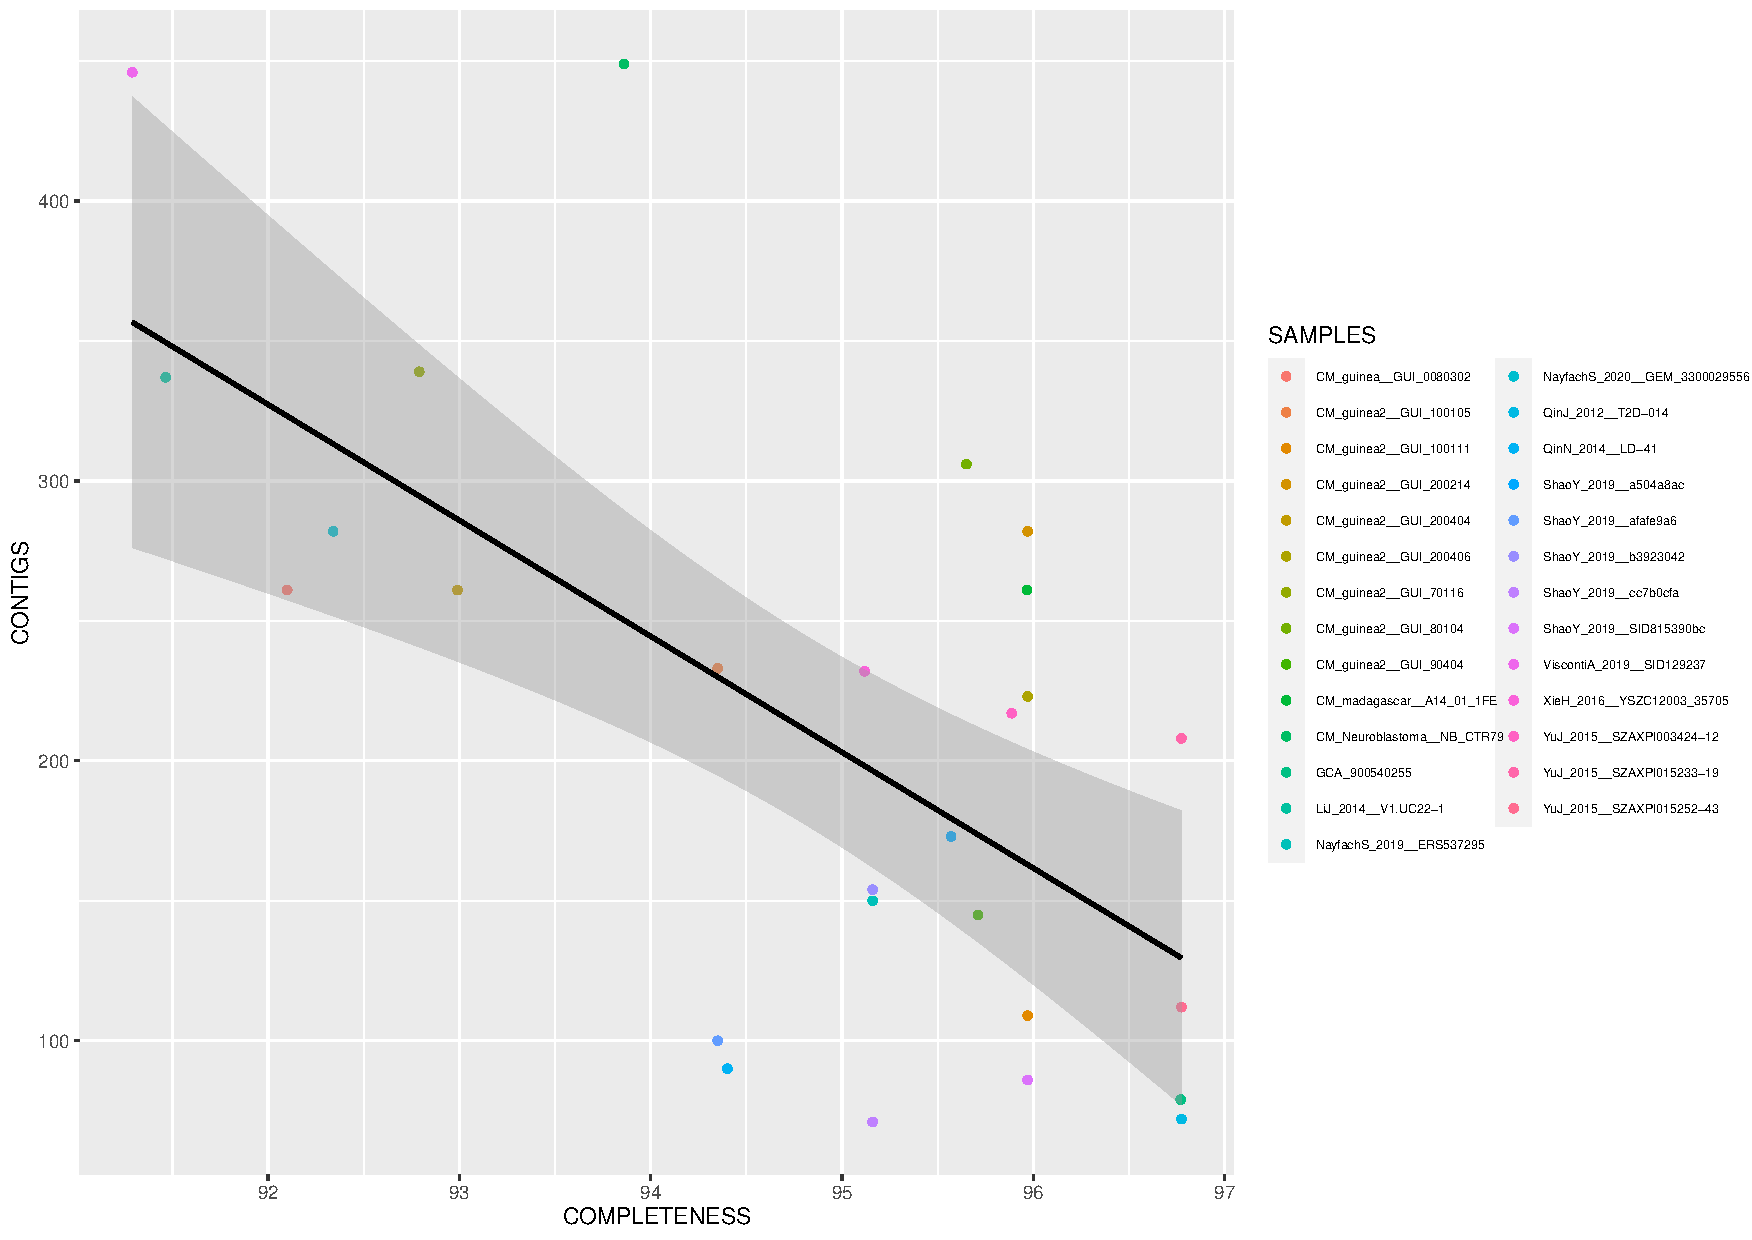
\includegraphics[width=1\linewidth]{ProjectCMG/images/CvC.pdf}
     \caption{Contigs versus Completeness per genome (MAG or isolate)}\label{fig:CvsC}
   %\end{minipage}\hfill
\end{figure}

\begin{figure}[!htb]
   %\begin{minipage}{0.6\textwidth}
     \centering
     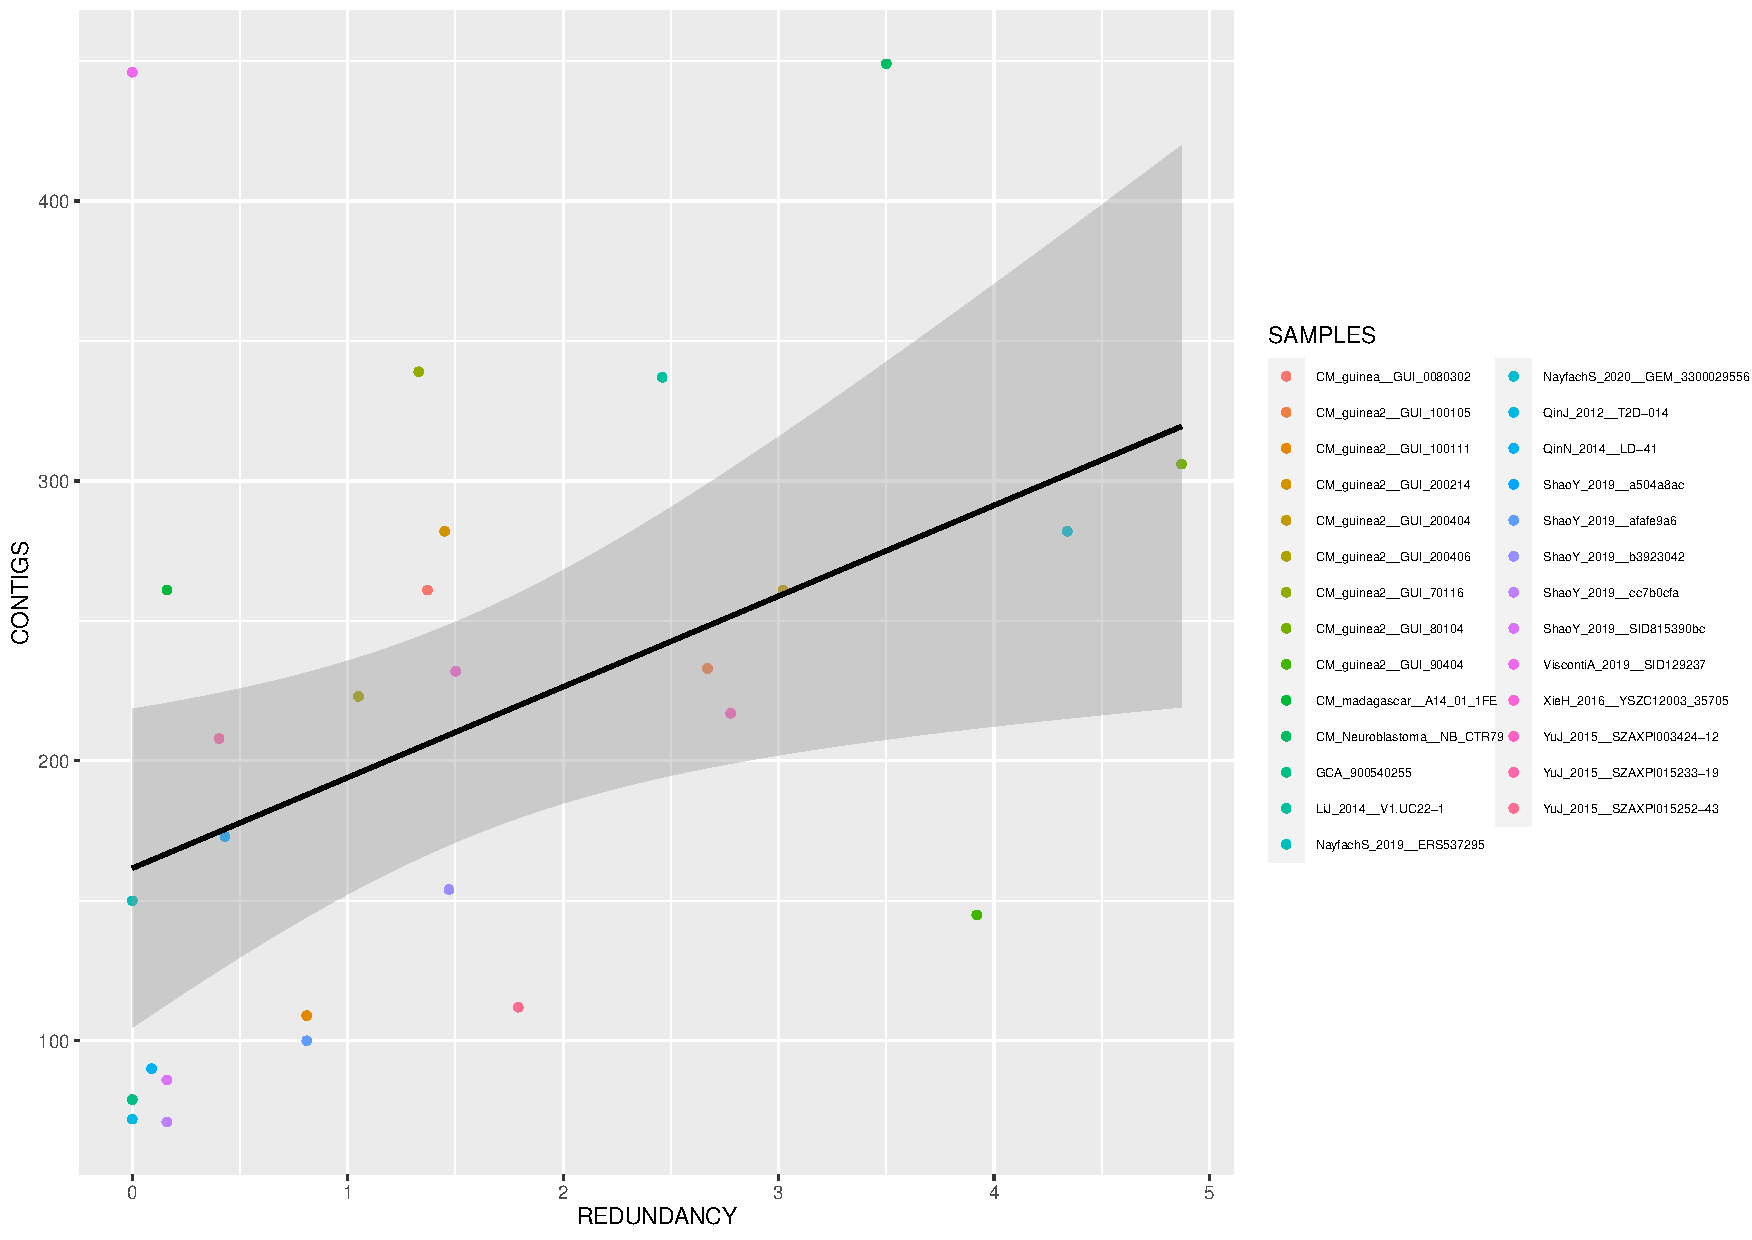
\includegraphics[width=1\linewidth]{ProjectCMG/images/CvR.pdf}
     \caption{Contigs versus Redundancy per genome (MAG or isolate)}\label{fig:CvsR}
   %\end{minipage}
\end{figure}

\begin{figure}[h!]
    \centering
    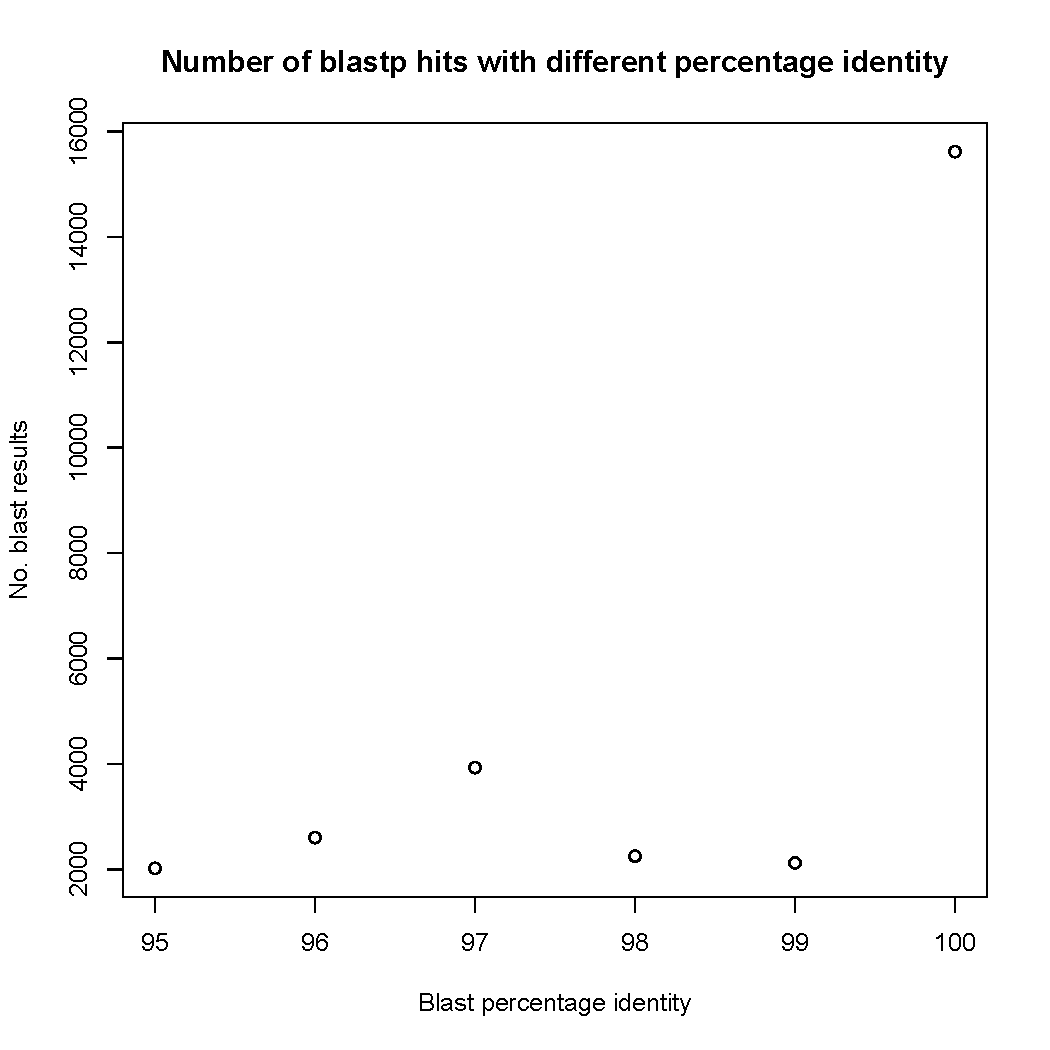
\includegraphics[width=.6\linewidth]{ProjectCMG/images/Rplot0.pdf}
    \caption{Number of Blastp hits with different percentage identity (using Blastp alignment)}
    \label{fig:roary1_1}    
\end{figure}

\begin{figure}[h!]
    \centering
    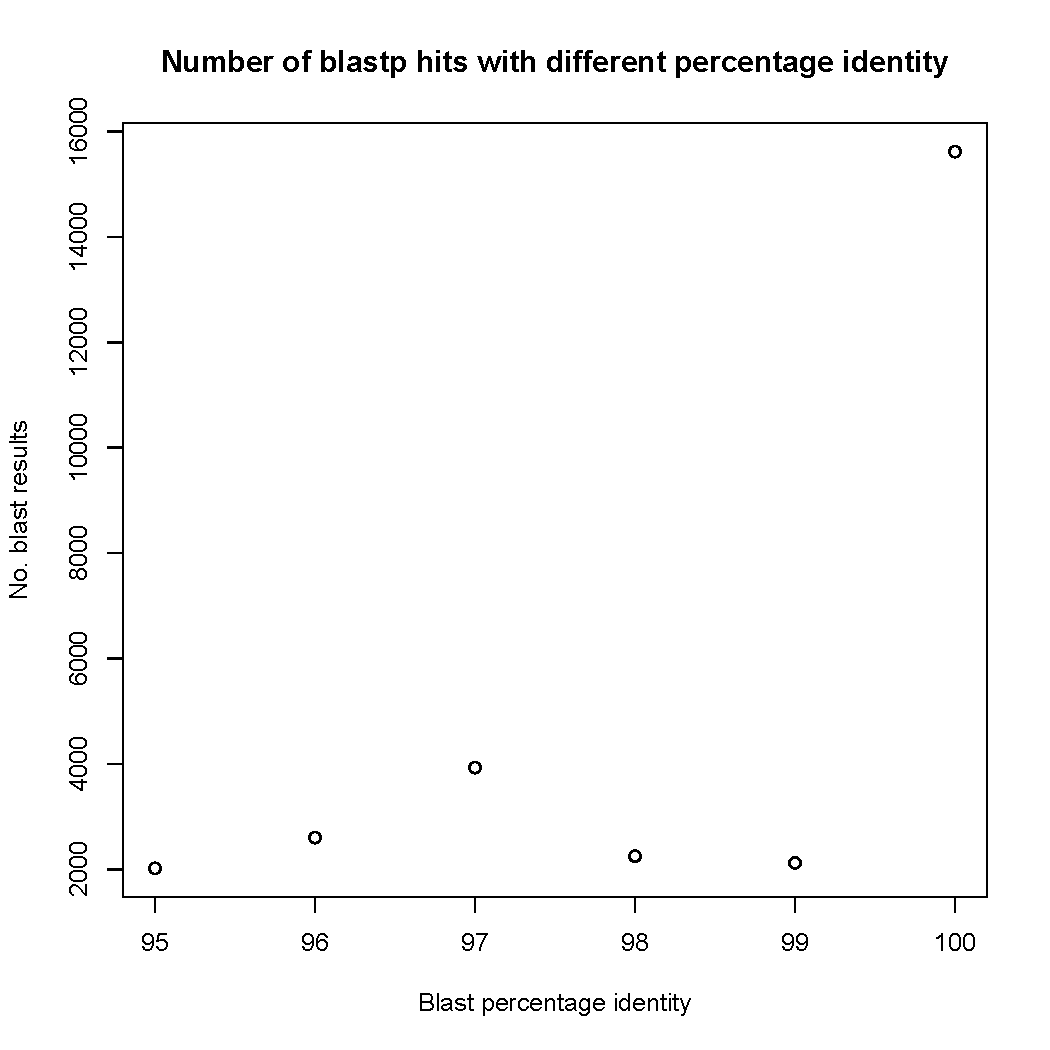
\includegraphics[width=.6\linewidth]{ProjectCMG/images/Rplot_new1.pdf}
    \caption{Number of Blastp hits with different percentage identity (using alignment with MAFFT and PRANK)}
    \label{fig:roary2_1}
    \end{figure}

\begin{figure}[!htb]
   \begin{minipage}{0.48\textwidth}
     \centering
     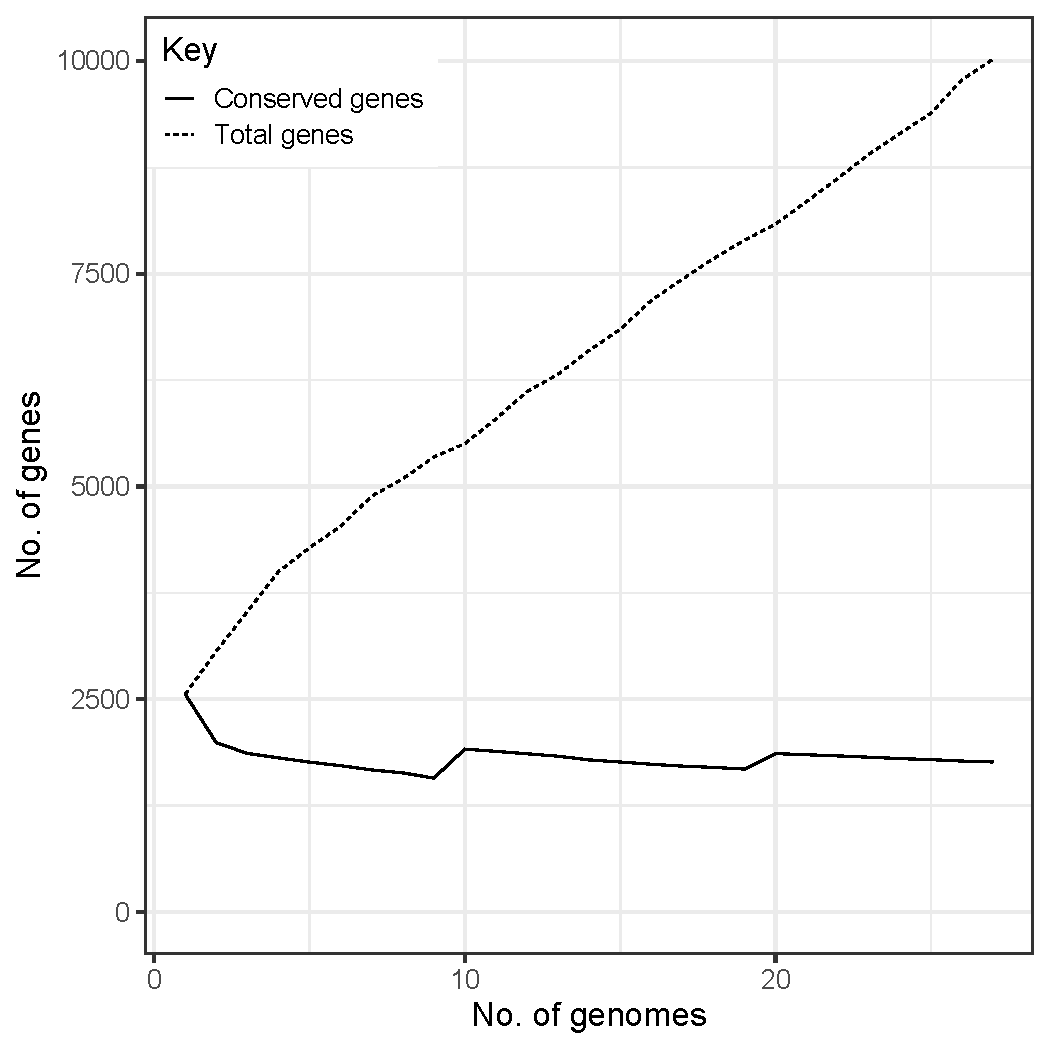
\includegraphics[width=.8\linewidth]{ProjectCMG/images/Rplot_new2.pdf}
     \caption{Conserved genes and total genes across pangenome: using alignment with MAFFT and PRANK}\label{fig:roary2_2}
   \end{minipage}\hfill
   \begin{minipage}{0.48\textwidth}
     \centering
     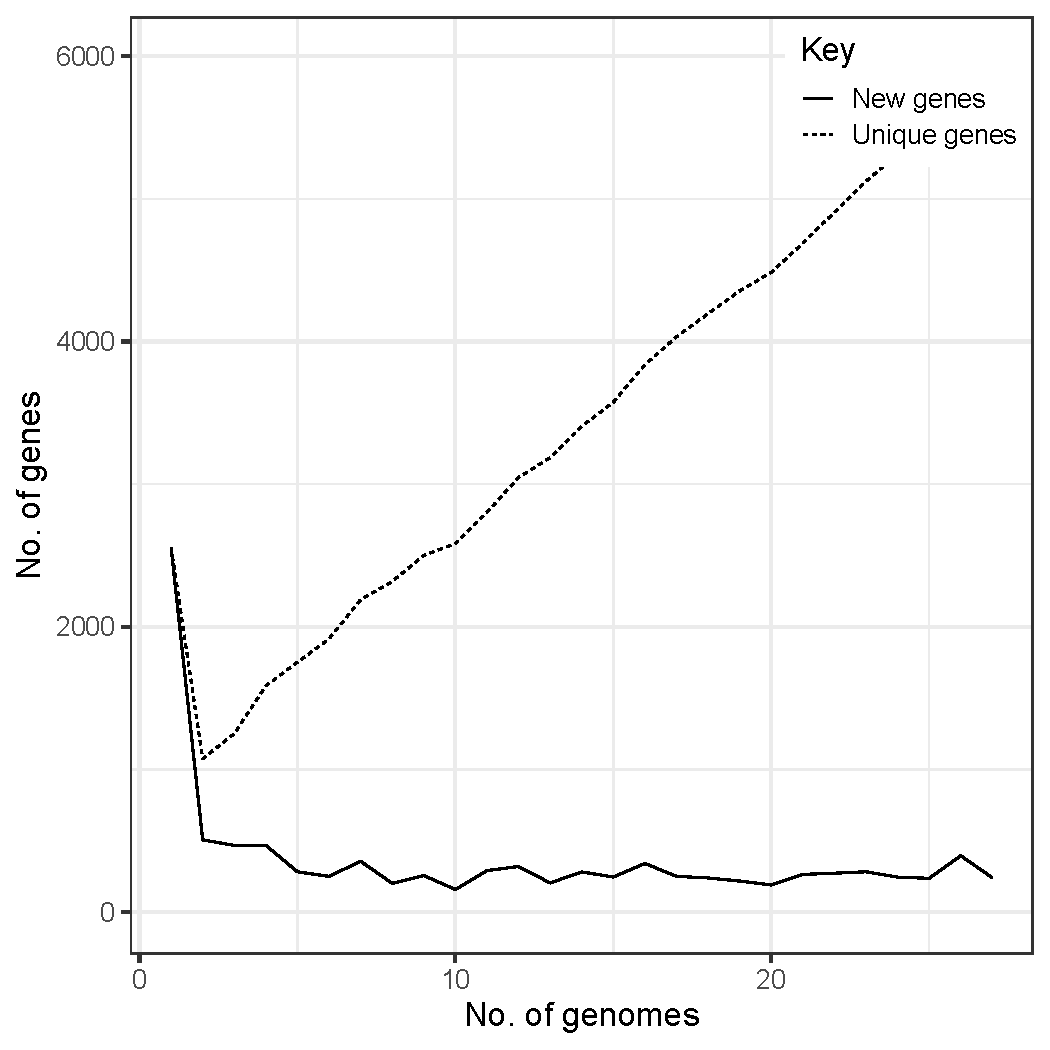
\includegraphics[width=.8\linewidth]{ProjectCMG/images/Rplot_new3.pdf}
     \caption{New genes and unique genes across pangenome (using alignment with MAFFT and PRANK)}\label{fig:roary2_3}
   \end{minipage}
\end{figure}

\begin{figure}
    \centering
    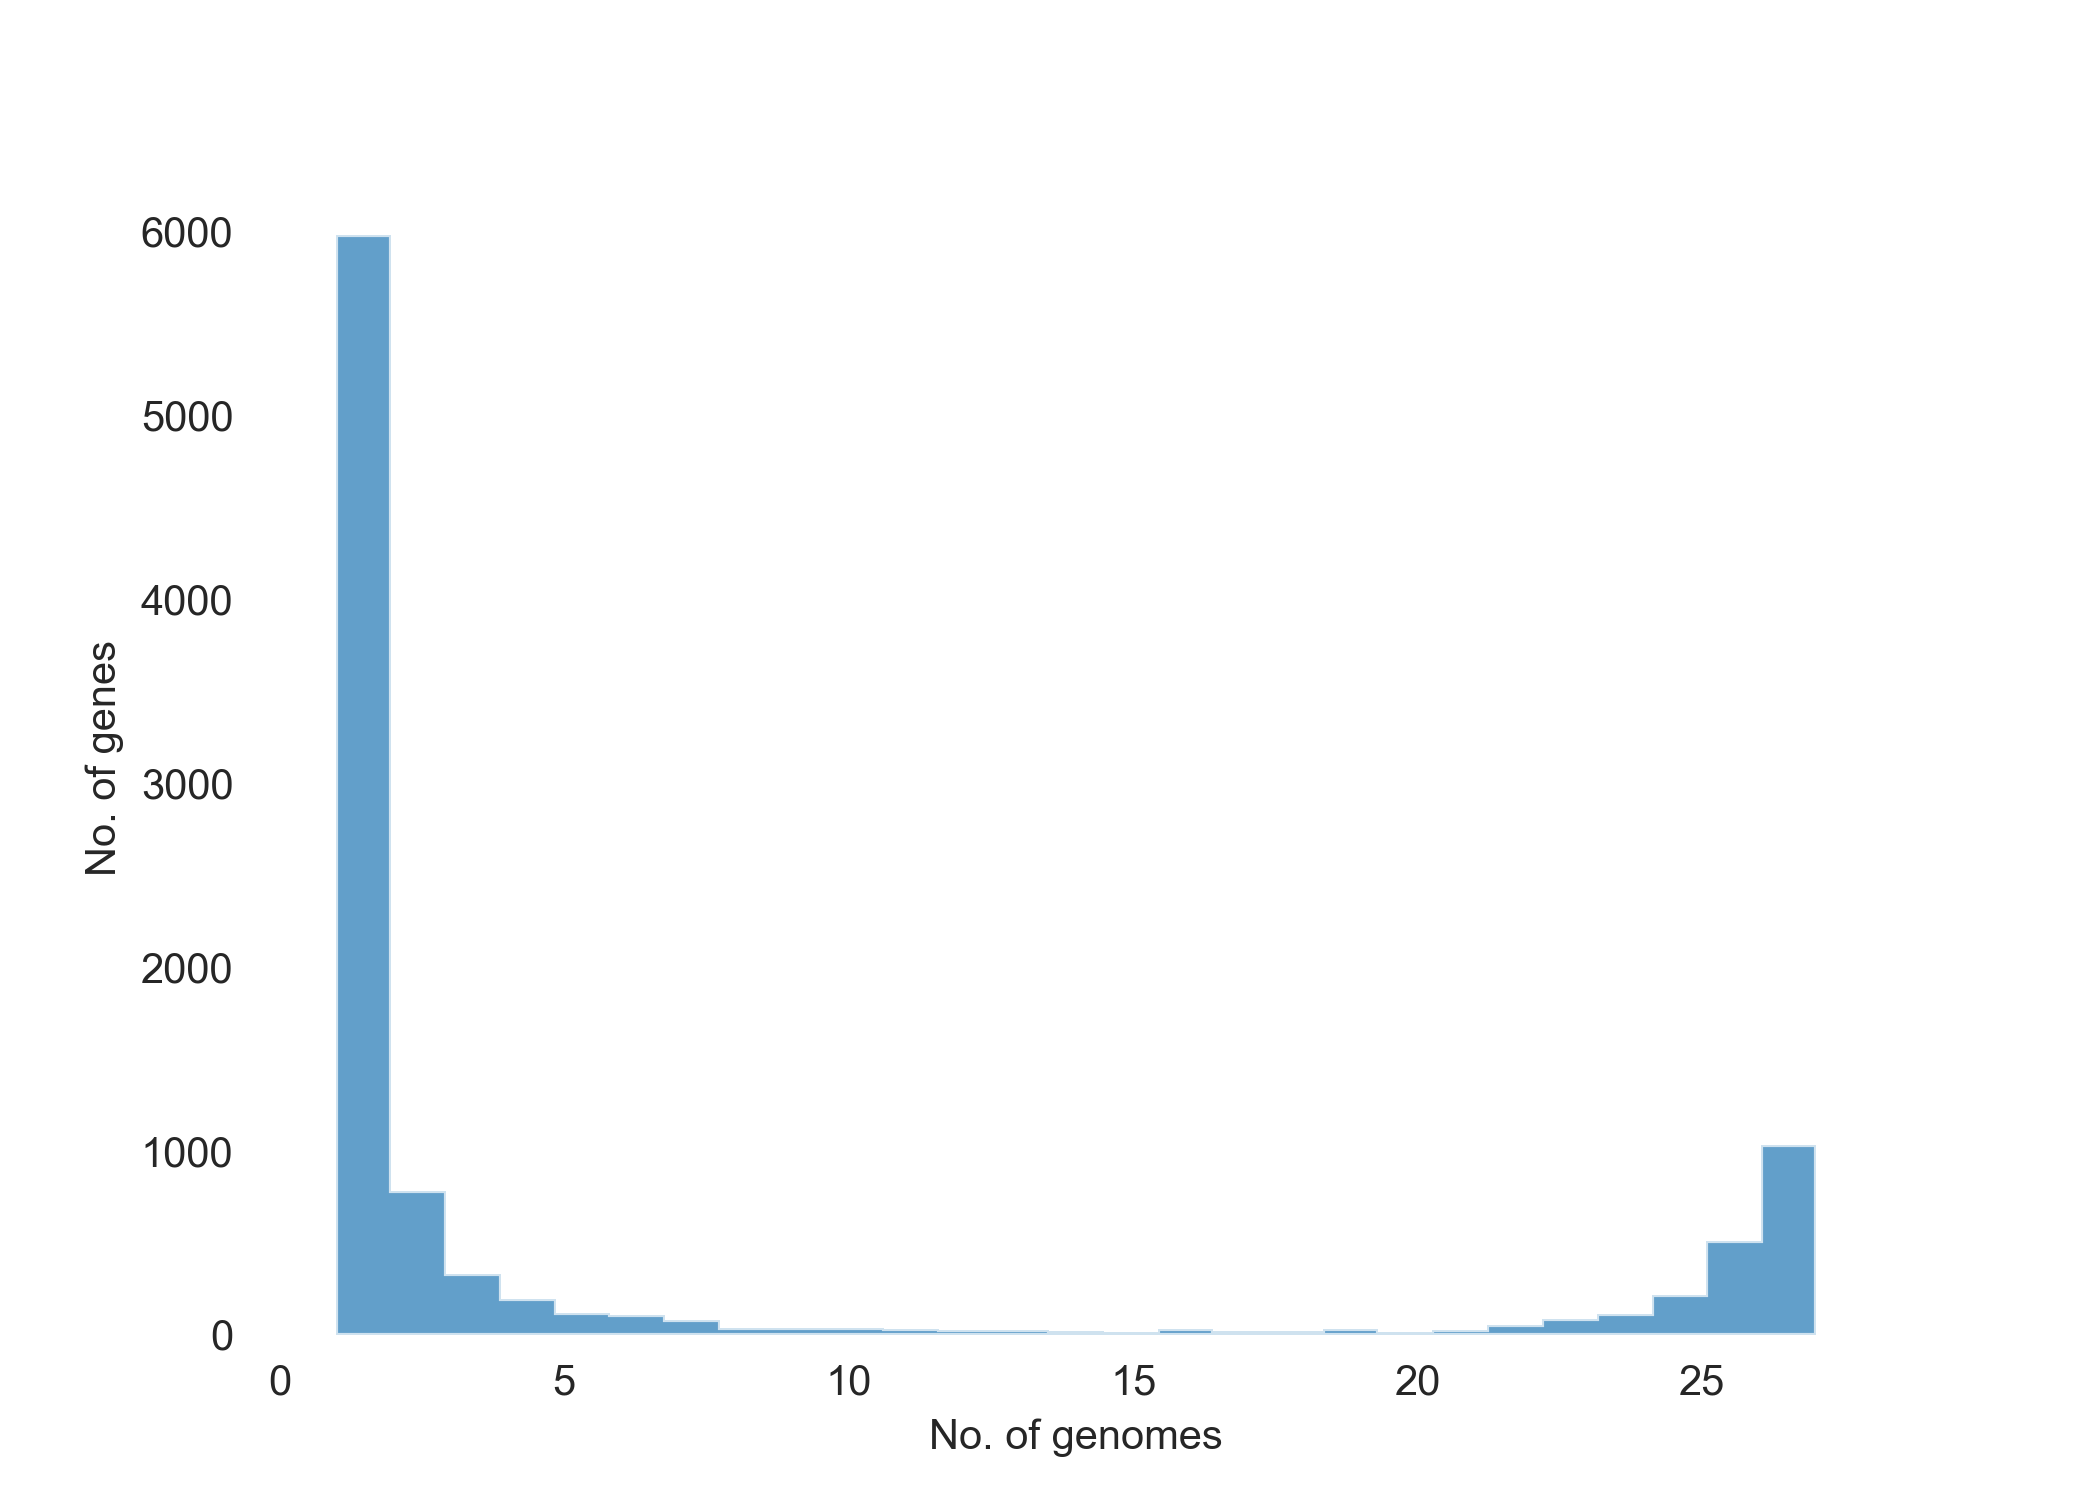
\includegraphics[width=.7\linewidth]{ProjectCMG/images/pangenome_frequency_new.png}
    \caption{Frequency of genes across pangenome (using alignment with MAFFT and PRANK)}\label{fig:roary2_freq}
\end{figure}


\begin{figure}
    \centering
    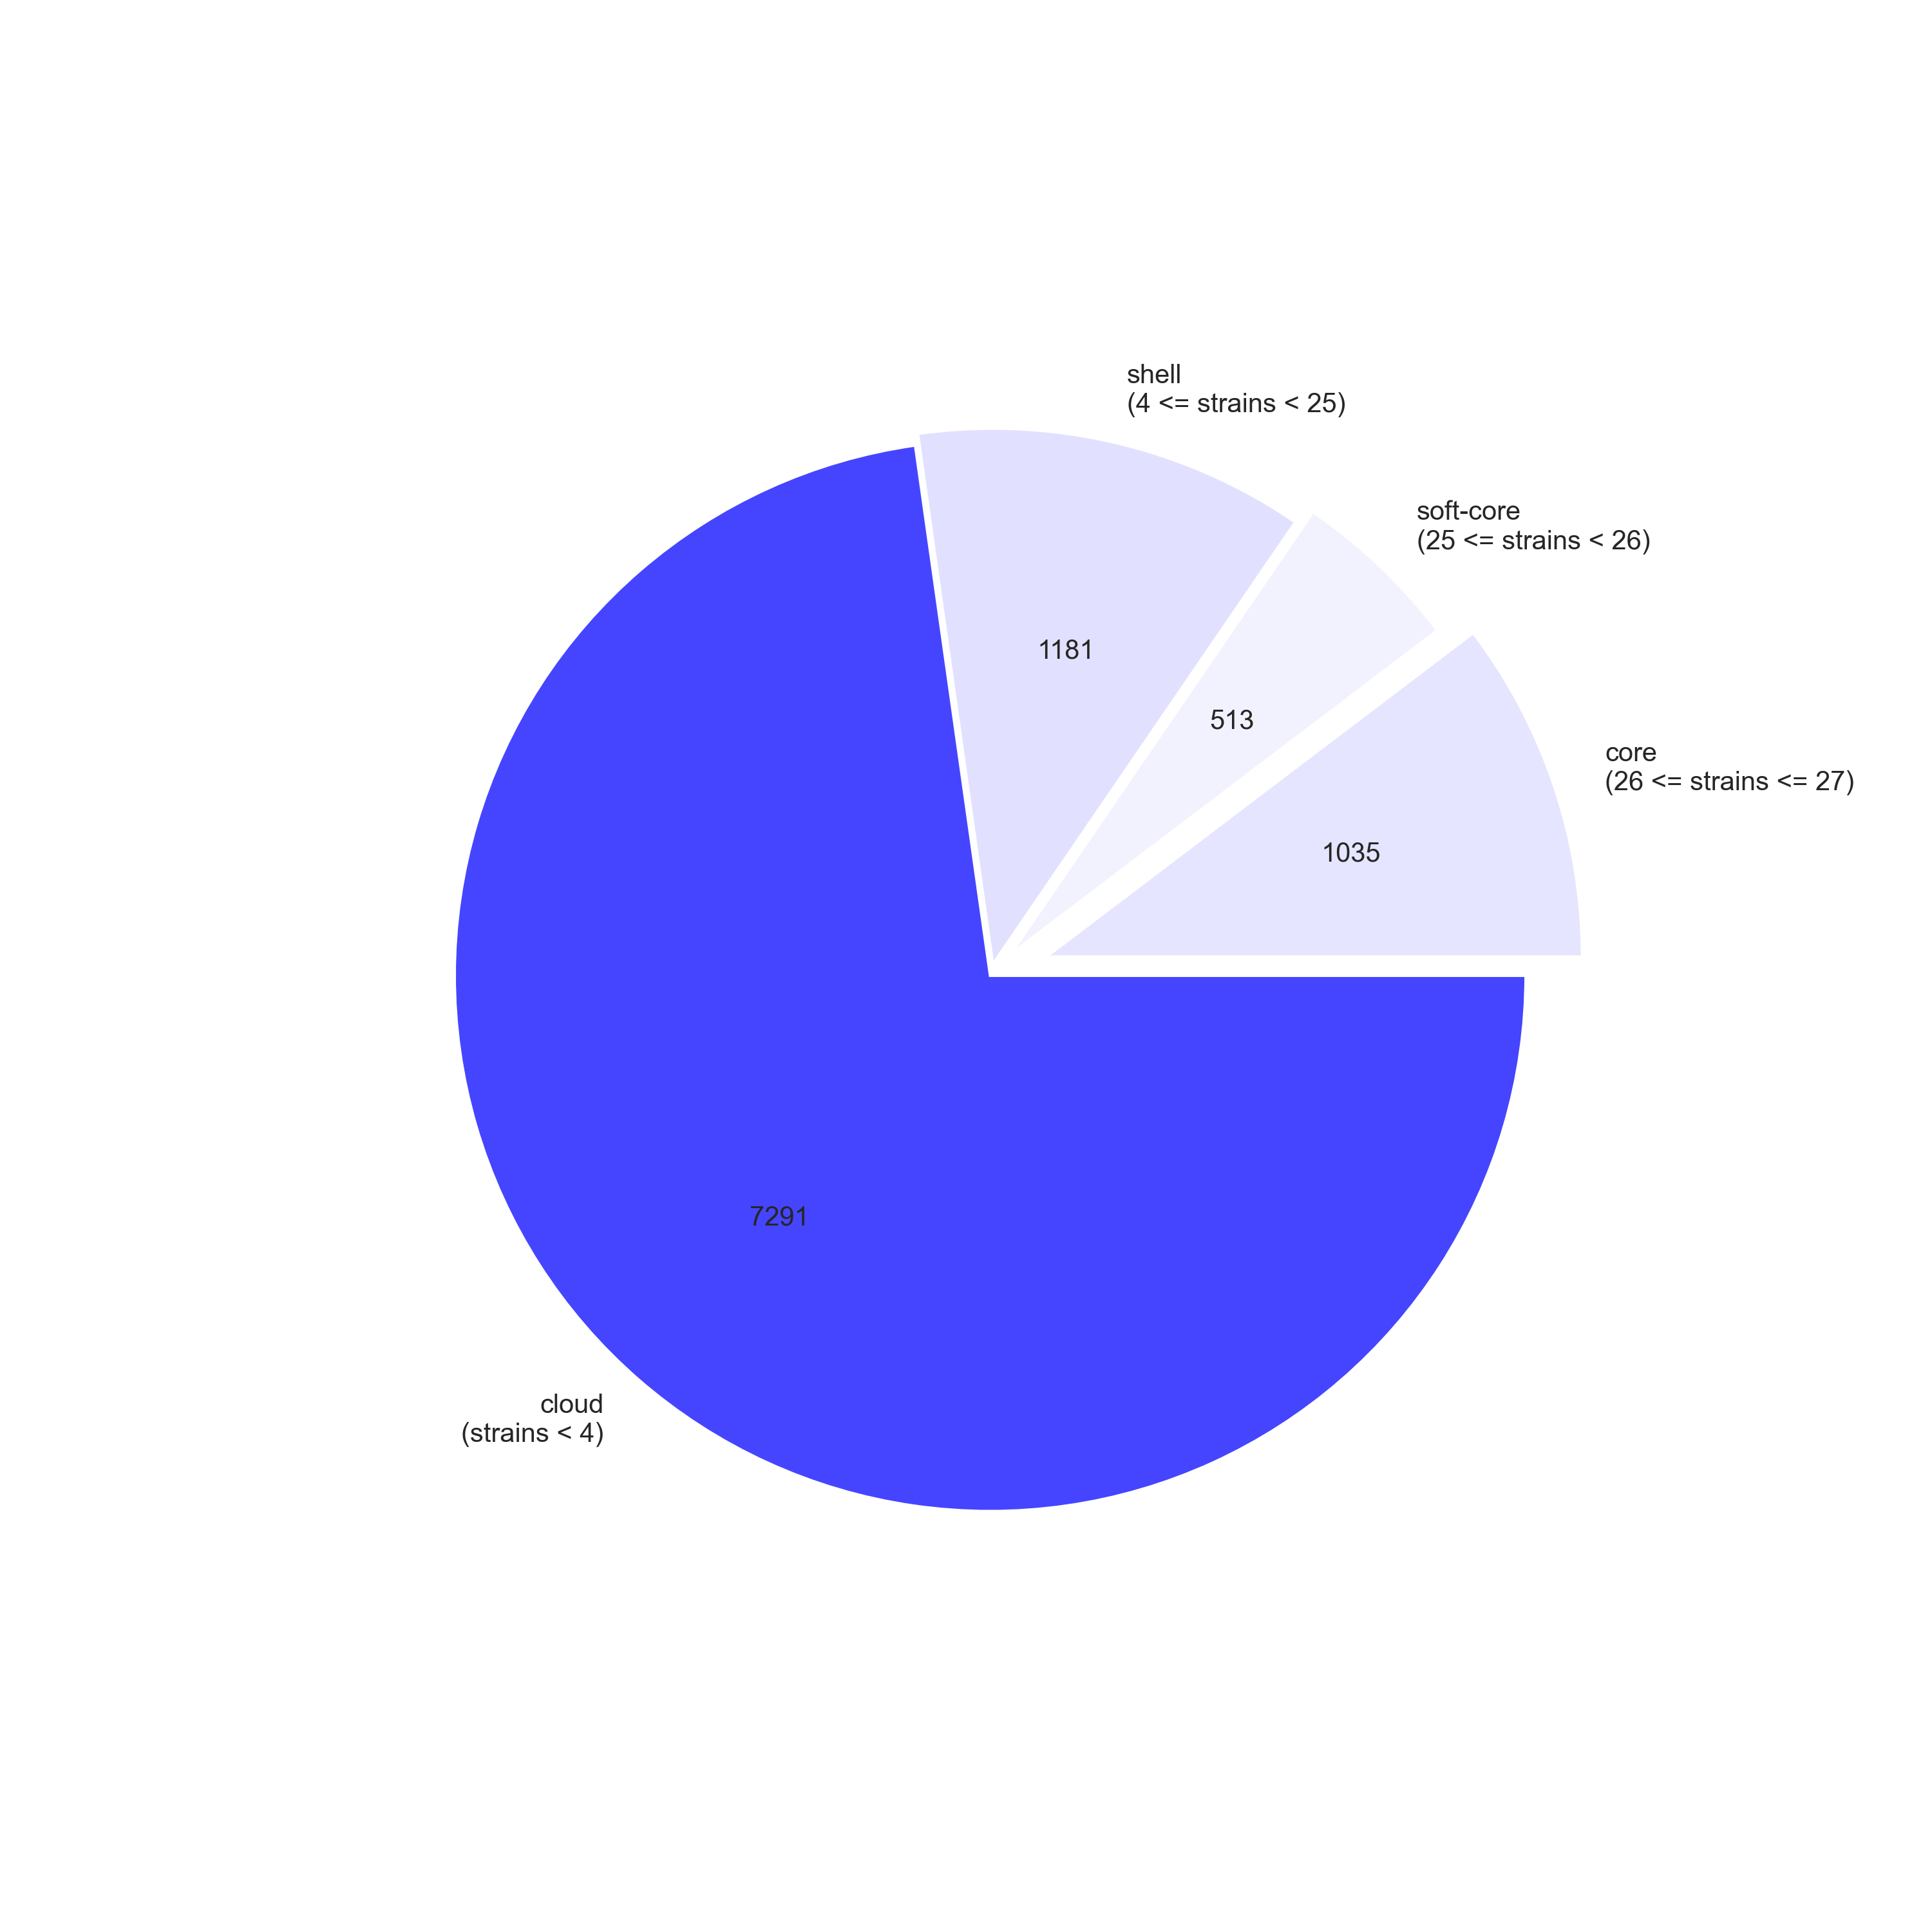
\includegraphics[width=\textwidth,height=\textheight,keepaspectratio]{ProjectCMG/images/pangenome_pie_new.png}
     \caption{Pangenome genes composition: cloud (7291), shell (1181), soft-core (513) and core (1035) genes (using alignment with MAFFT and PRANK)}\label{fig:roary2_pie}
\end{figure}

\begin{figure}[h!]
    \centering
    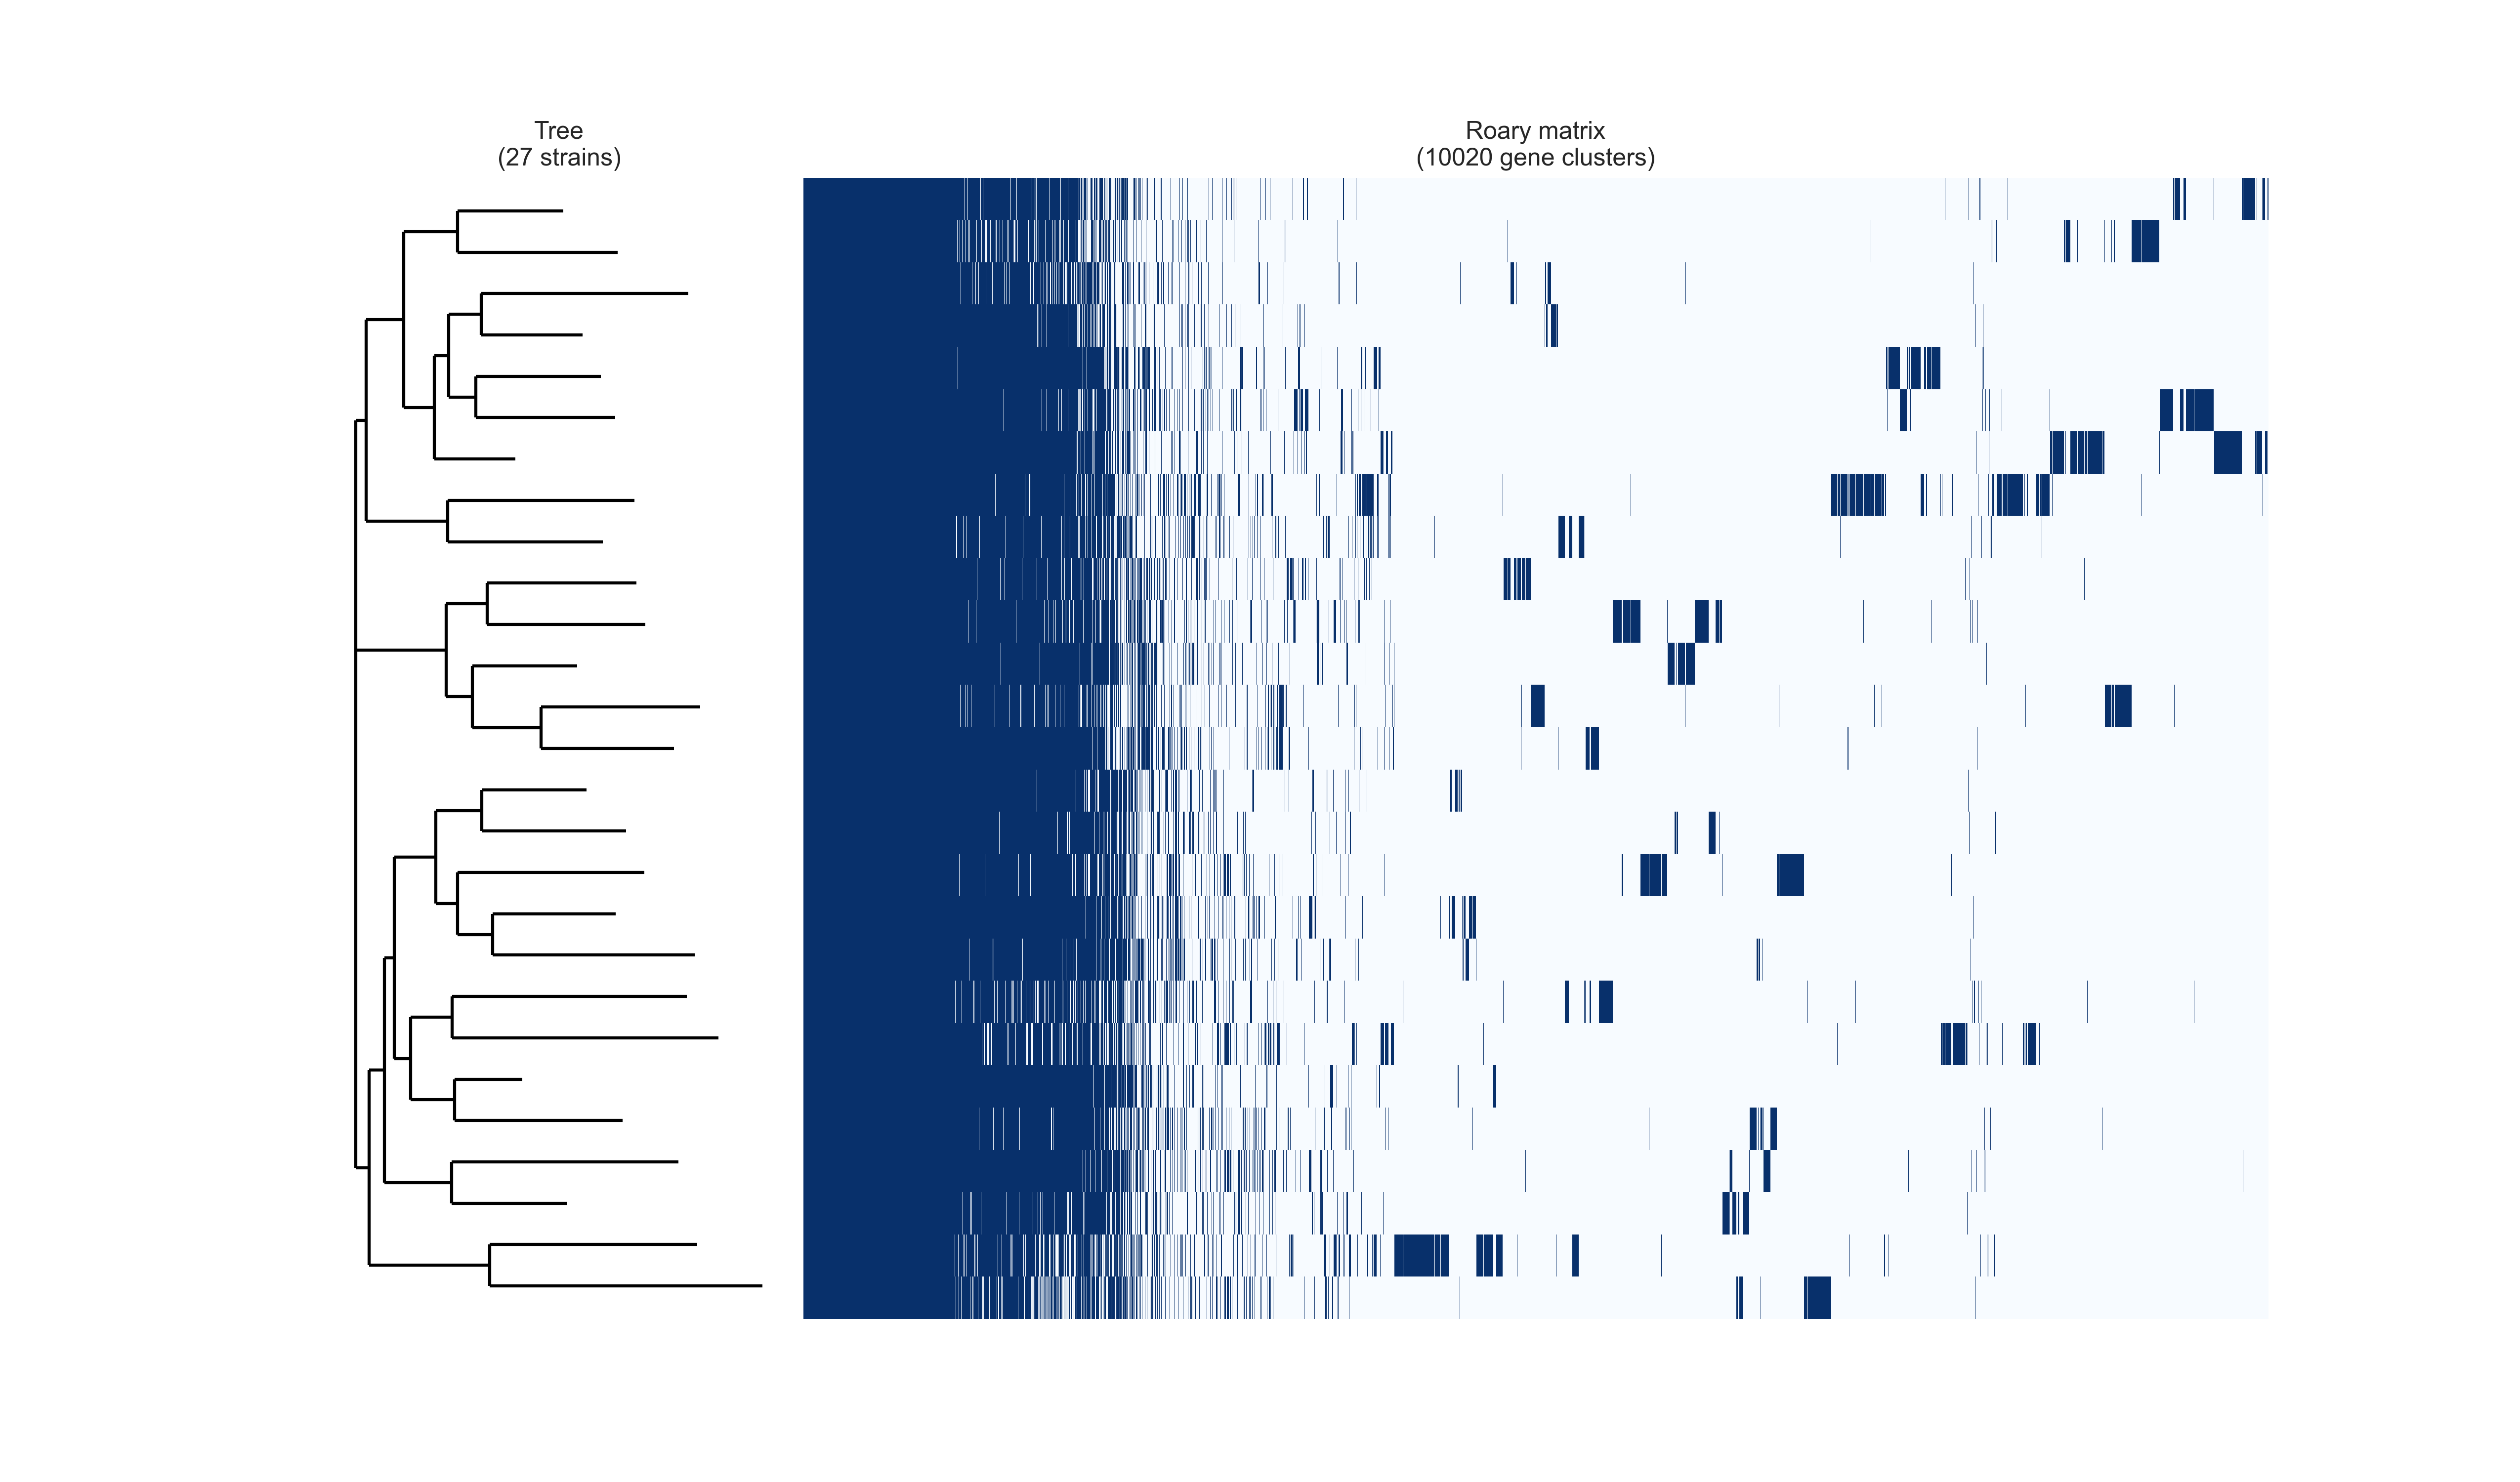
\includegraphics[width=1.2\linewidth]{ProjectCMG/images/pangenome_matrix_new.png}
    \caption{Heatmap of pangenome (using alignment with MAFFT and PRANK). Dark blue represents gene presence; light blue represents gene absence.The x-axis represents 10020 genes clusters and y-axis represents 27 strains in dendrogram. The gene clusters at left in dark blue depicts core genes.}
    \label{fig:roary2_matrix}
\end{figure}

\begin{landscape}
\begin{table}[!ht]
    \centering
    \begin{tabular}{|l|l|}
    \hline
        \#input\_bin & uSGB taxonomical distance \\ \hline
        CM\_madagascar\_\_A14\_01\_1FE\_\_bin.13 & uSGB\_6179|t\_\_SGB6179: 0.01834493125 \\ \hline
        LiJ\_2014\_\_V1.UC22-1\_\_bin.24 & uSGB\_6179|t\_\_SGB6179: 0.01812152649193548 \\ \hline
        QinJ\_2012\_\_T2D-014\_\_bin.33 & uSGB\_6179|t\_\_SGB6179: 0.015865366411290324 \\ \hline
        QinN\_2014\_\_LD-41\_\_bin.25 & uSGB\_6179|t\_\_SGB6179: 0.015955060927419357 \\ \hline
        XieH\_2016\_\_YSZC12003\_35705\_\_bin.27 & uSGB\_6179|t\_\_SGB6179: 0.019111369879032256 \\ \hline
        YuJ\_2015\_\_SZAXPI003424-12\_\_bin.14 & uSGB\_6179|t\_\_SGB6179: 0.02015145318548387 \\ \hline
        YuJ\_2015\_\_SZAXPI015233-19\_\_bin.67 & uSGB\_6179|t\_\_SGB6179: 0.01643216536290323 \\ \hline
        YuJ\_2015\_\_SZAXPI015252-43\_\_bin.58 & uSGB\_6179|t\_\_SGB6179: 0.01823083766129032 \\ \hline
        CM\_guinea2\_\_GUI\_100105\_\_bin.75 & uSGB\_6179|t\_\_SGB6179: 0.02398411612903226 \\ \hline
        CM\_guinea2\_\_GUI\_100111\_\_bin.34 & uSGB\_6179|t\_\_SGB6179: 0.019066705887096774 \\ \hline
        CM\_guinea2\_\_GUI\_200214\_\_bin.86 & uSGB\_6179|t\_\_SGB6179: 0.019749577943548386 \\ \hline
        CM\_guinea2\_\_GUI\_200404\_\_bin.54 & uSGB\_6179|t\_\_SGB6179: 0.01768373052419355 \\ \hline
        CM\_guinea2\_\_GUI\_200406\_\_bin.2 & uSGB\_6179|t\_\_SGB6179: 0.021495570564516127 \\ \hline
        CM\_guinea2\_\_GUI\_70116\_\_bin.90 & uSGB\_6179|t\_\_SGB6179: 0.01877004794354839 \\ \hline
        CM\_guinea2\_\_GUI\_80104\_\_bin.57 & uSGB\_6179|t\_\_SGB6179: 0.01979633435483871 \\ \hline
        CM\_guinea2\_\_GUI\_90404\_\_bin.43 & uSGB\_6179|t\_\_SGB6179: 0.01611623120967742 \\ \hline
        CM\_guinea\_\_GUI\_0080302\_\_bin.8 & uSGB\_6179|t\_\_SGB6179: 0.017641257741935482 \\ \hline
        CM\_Neuroblastoma\_\_NB\_CTR79\_\_bin.26 & uSGB\_6179|t\_\_SGB6179: 0.01964306290322581 \\ \hline
        GCA\_900540255 & uSGB\_6179|t\_\_SGB6179: 0.017724237499999997 \\ \hline
        NayfachS\_2019\_\_ERS537295\_\_bin.57 & uSGB\_6179|t\_\_SGB6179: 0.019090847177419355 \\ \hline
        NayfachS\_2020\_\_GEM\_3300029556\_\_bin.6 & uSGB\_6179|t\_\_SGB6179: 0.023584942983870965 \\ \hline
        ShaoY\_2019\_\_a504a8ac-7ae6-11e9-a106-68b59976a384\_\_bin.8 & uSGB\_6179|t\_\_SGB6179: 0.016583730443548387 \\ \hline
        ShaoY\_2019\_\_afafe9a6-7ae6-11e9-a106-68b59976a384\_\_bin.6 & uSGB\_6179|t\_\_SGB6179: 0.017236076975806452 \\ \hline
        ShaoY\_2019\_\_b3923042-7ae6-11e9-a106-68b59976a384\_\_bin.23 & uSGB\_6179|t\_\_SGB6179: 0.01742517806451613 \\ \hline
        ShaoY\_2019\_\_cc7b0cfa-7ae6-11e9-a106-68b59976a384\_\_bin.21 & uSGB\_6179|t\_\_SGB6179: 0.018078696693548384 \\ \hline
        ShaoY\_2019\_\_SID815390bc-7ae6-11e9-a106-68b59976a384\_\_bin.19 & uSGB\_6179|t\_\_SGB6179: 0.01674633721774194 \\ \hline
        ViscontiA\_2019\_\_SID129237\_\_bin.45 & uSGB\_6179|t\_\_SGB6179: 0.019415520564516127 \\ \hline
    \end{tabular}
    \caption{Taxonomical distances of MAGs and \textit{Clostridium} isolate. Kingdom: Bacteria, Phylum: Firmicutes, Class: Clostridia, Order: Clostridiales, Family: Clostridiaceae, Genus: Clostridium, Species: Clostridium\_SGB6179.}
    \label{Table:Taxonomical distance of MAGs}
\end{table}
\end{landscape}

\end{document}


%%%%%%%%%%%%%%%%%%%%%%%%%%%%%%%%%%%%%%%%%%%%%%%%%%%%%%%%%%%%%%%%%%%%%%%%%%%%%%%%%%%%%

% Here are some equations and other useful things, feel free to copy and paste into your lab report :) %

% Note: It is super easy to look up equations/constants already formatted in LaTeX online. Here are a few websites I like to use:

% LaTeX Tutorial: http://pages.physics.cornell.edu/sps/pages/resources/latex.html
	%NOTE: This contains both pdf and text (code) of each document, which includes guides, lab 			report templates, and lots of other good stuff!

% LaTeX Cheat Sheet: http://wch.github.io/latexsheet/

% Equations: http://www.equationsheet.com/sheets/Equations-5.html

% Constants, symbols, letters, etc:  http://www.rpi.edu/dept/arc/training/latex/LaTeX_symbols.pdf

% AP Physics Calculus Reference Table: https://secure-media.collegeboard.org/digitalServices/pdf/ap/physics-c-tables-and-equations-list.pdf

% AP Physics Trig Reference Table: https://secure-media.collegeboard.org/digitalServices/pdf/ap/ap-physics-1-equations-table.pdf

% Regents Physics Reference Table: http://www.p12.nysed.gov/assessment/reftable/physics-rt/physics06tbl.pdf

% Here are three good sources to use other then this for considering how to write a good lab report. Much of this guide was gleaned from them
	% http://pages.physics.cornell.edu/sps/pages/resources/LatexSession/Exercises/LabReport.pdf -Cornell Template
    % http://physics.columbia.edu/files/physics/content/1291_report_format_and_example.pdf 		-Columbia University Template
    % https://www.baylor.edu/physics/doc.php/110769.pdf											-Baylor University Template
    % www.nd.edu/~hgberry/Fall2012/Guidelines.docx												-Notre Dame Template
    %http://www.esf.edu/iq/colloquium/documents/LabReportnotes.pdf								-SUNY ESF Template
    %http://writing.engr.psu.edu/workbooks/laboratory.html										-Virginia Tech Template
    %https://projects.ncsu.edu/labwrite/index_labwrite.htm										-SUPER in-depth guide to writing lab reports
    
    %https://gist.github.com/dcernst/1827406													-Template for completing Math homework in LaTeX
    %https://joshldavis.com/2014/02/12/doing-your-homework-in-latex/							-More about math homework in LaTeX
    
    
    
%Purdue University Online Writing Lab-OWL: https://owl.english.purdue.edu/ Use this to generate citations!

%Basically, if you get stuck, just google "Latex ______" for whatever you need and look through the LaTeX stackexchange or wiki article to find and copy/paste what you need





%	Here are some common equations we use in class. I will continue to update as we continue throughout the year. I will attempt to organize by the order we learn the topics from oldest at the top to newest at the bottom. 

%%%%%%%%%%%%%%%%%%%%%%%%%% Basic Calculus %%%%%%%%%%%%%%%%%%%%%%%%%%%%%%%%%%%%%

%		   $$\frac{\mathrm{d}}{\mathrm{d}x}C=0$$
%           $$\frac{\mathrm{d}}{\mathrm{d}x}Cx=C$$
%           $$\frac{\mathrm{d}}{\mathrm{d}x}x=1$$           
%           $$\frac{\mathrm{d}}{\mathrm{d}x}x^n = nx^{n-1} $$  	-power rule
% 		   $$\frac{\mathrm{d}}{\mathrm{d}x}fg= fg'+f'g$$		-product rule
%           $$\frac{\mathrm{d}}{\mathrm{d}x}f(g(x))=f'(g(x))g'(x)$$	-chain rule
%           $$\frac{\mathrm{d}}{\mathrm{d}x} \sin{x} = \cos{x}$$	
%           $$\frac{\mathrm{d}}{\mathrm{d}x} \cos{x} = -\sin{x}$$
           
%           $$\int k \mathrm{d}x = kx+C$$		-integral of a constant
%           $$\int x^n \mathrm{d}x= \frac{1}{n+1}x^{n+1}+C$$	-power rule for integrals
%           $$\int \cos{u}\mathrm{d}u = \sin{u} + C$$	
%           $$\int \sin{u}\mathrm{d}u = -cos{u} + C$$	

% see https://reu.dimacs.rutgers.edu/Symbols.pdf for a nice list of math LaTeX symbols

%%%%%%%%%%%%%%%%%%%%%%%%%%%%  Kinematics %%%%%%%%%%%%%%%%%%%%%%%%%%%%%%%%%%%%%%%

%			$$\bar{v}=\frac{d}{t}$$ 								-average speed
%			$$v=\frac{\mathrm{d}x}{\mathrm{d}t}$$					-instantaneous velocity definition
%			$$a=\frac{\mathrm{d}v}{\mathrm{d}t}$$					-instantaneous acceleration definition
%			if acceleration is constant, then:
%				$${x_f}={x_i}+{v_i}t+\frac{1}{2}a{t^2}$$  			-free-fall equation
%				$${v_f}={v_i}+at$$									-find new velocity
%				$${{v_f}^2}={{v_i}^2}+2a({x_f}-{x_i})$$				-equation without time

%%%%%%%%%%%%%%%%%%%%%%%%%%%%% Newton's Laws %%%%%%%%%%%%%%%%%%%%%%%%%%%%%%%%%%%%%%

%			$$F_{net}=ma=m\frac{\mathrm{d}v}{\mathrm{d}t}=m\frac{\mathrm{d}^{2}x}{\mathrm{d}{t^2}}$$	-Newt's 2nd Law
%			$$F_f=\mu F_n$$											-Friction 
%			$$w=mg$$												-Weight

%%%%%%%%%%%%%%%%%%%%%%%%%%%%%%%% Work, Power, Energy %%%%%%%%%%%%%%%%%%%%%%%%%%%%%%%%%%%

%			$$W=\Delta E = \int F dx = Fd  \hspace{3pt} \text{(if F constant)} $$ 	-Work-Energy Theorem
%			$$Power=\frac{\mathrm{d}E}{\mathrm{d}t}=\frac{\mathrm{d}W}{\mathrm{d}t} = \frac{Fd}{t} = F \bar{v}$$		-Power
%			$$K=\frac{1}{2}mv^2$$													-Kinetic Energy
%			$$U_g=mgh$$																-Gravitational Potential Energy
%			$$U_e=\frac{1}{2}kx^2$$													-Spring Potential Energy
%			$$F_e=kx$$																-Hooke's Law
%			$$F=-\frac{\mathrm{d}U}{\mathrm{d}x}$$									-Force is derivative of Potential

%%%%%%%%%%%%%%%%%%%%%%%%%%%%%%%%%%%%% Momentum, Center of Mass %%%%%%%%%%%%%%%%%%%%%%%%%%%%%%%%%%%

% 			$$p=mv$$								-definition of momentum
%			$$F=\frac{\mathrm{d}p}{\mathrm{d}t}
%			$$ft=\Delta{p}$$ 						-trig version of impulse momentum theorem
%			$$J=\int F \mathrm{d}t = \Delta{p}$$	-calc version of impulse momentum theorem
%			$$p_{before}=p_{after}$$				-Conservation of Momentum
%			$$X_{c.o.m}=\frac{\Sigma x_i m_i}{M}$$  -x-coordinate of Center of Mass
%       	$$Y_{c.o.m}=\frac{\Sigma y_i m_i}{M}$$  -y-coordinate of Center of Mass


%%%%%%%%%%%%%%%%%%%%%%%%%%%%%%%%%%% Rotational Kinematics %%%%%%%%%%%%%%%%%%%%%%%%%%%%%%%%%%%%%%%

%		$$\omega=\frac{\mathrm{d}\theta}{\mathrm{d}t}$$ 			-definition of angular speed (rad/sec)
%		$$\alpha=\frac{\mathrm{d}\omega}{\mathrm{d}t}=\frac{\mathrm{d}^2\theta}{\mathrm{d}t^2}$$ 			-definition of angular acceleration
%		$$v=r\omega$$												-angular/linear velocity connection
%		$$S=r \theta$$												-arc length/angle connection
%		if angular acceleration is constant, then:
%			$$\omega_f=\omega_i+\alpha t$$   	-find angular velocity
%			$$\theta=\theta_i + \omega_i t + \frac{1}{2} \alpha t^2$$ 		-angular "free-fall" equation
%			$${\omega_f}^2 = {\omega_i}^2 + 2\alpha(\theta_f - \theta_i)$$ 	-angular equation w/o time

%%%%%%%%%%%%%%%%%%%%%%%%%%%%%%%% Rotational Dynamics + Gravitation %%%%%%%%%%%%%%%%%%%%%%%%%%%%%%%%%%%%%%%%%%%

%		$$\tau=r \times F = rF\sin{\theta}$$			-definition of torque
%		$$\tau = I \alpha$$								-Newt's 2nd Law for Rotation
%		$$a_c = v^{2}/r = {\omega^2}r$$					-centripetal acceleration
%		$$F_c=ma_c = m{\omega^2}r$$						-centripetal force
%		$$I=\int r^2 \mathrm{d}m = \Sigma m r^2$$		-Calculate Moment of Inertia of an Object
%		$$K_r=\frac{1}{2}I{\omega^2}$$					-Rotational Kinetic Energy
%		$$L= I\omega = r \times p = rp\sin{\theta}$$	-Angular Momentum
%		$$L_{before}=L_{after}$$						-Conservation of Angular Momentum

%		$$F_g = \frac{\text{G}m_1 m_2}{r^2}$$			-Newton's Law of Universal Gravitation
%		$$U_g= -\frac{\text{G}m_1 m_2}{r}$$				-Gravitational Potential Energy

%%%%%%%%%%%%%%%%%%%%%%%%% Vibrations, Simple Harmonic Motion, Sound %%%%%%%%%%%%%%%%%%%%%%%%%%%%%%	

%		$$v=f\lambda$$								-speed of a wave
%		$4T=\frac{2\pi}{\omega}=\frac{1}{f}$$		-period of a wave
%		$$x(t)=x_{max}\cos{(\omega t + \phi)}$$	    -wave equation
%		$$T_s=2\pi\sqrt{\frac{m}{k}}$$				-Period of an oscillating spring
%		$$T_p=2\pi\sqrt{\frac{l}{g}}$$				-Period of a Pendulum
%		$$\frac{\mathrm{d}^2 \smiley{}}{{dt}^2} - {\omega}^2 \smiley{} = 0$$ 	-General Simple Harmonic Motion Equation
%		
		
%%%%%%%%%%%%%%%%%%%%%%%%%%%%%%%%%%%%%% Fluid Mechanics %%%%%%%%%%%%%%%%%%%%%%%%%%%%%%%%%%%%%%%%%%%

%		$$\rho=m/V$$						-Density
%		$$P=F/A$$							-Definition of Pressure
%		$$P=P_i+\rho gh	$$					-Pressure change as a function of depth
%		$$\rho_1A_1v_1=\rho_2A_2v_2$$		-Continuity Equation for fluid flow
%		$$F_b=\rho gV_{displaced}$$			-Archimedes Principle
%		$$P_1+\frac{1}{2}\rho v_1^2 +\rho gh_1 = P_2+\frac{1}{2}\rho v_2^2 +\rho gh_2 $$ -Bernoulli Equation
%		

%%%%%%%%%%%%%%%%%%%%%%%%%%%%%%%%%%%%%% Thermodynamics %%%%%%%%%%%%%%%%%%%%%%%%%%%%%%%%%%%%%%%%%%%%%

%		$$\frac{\Delta Q}{\Delta t} = \frac{k A \Delta T}{l}$$ 		-Conduction Equation
%		$$Q = mc \Delta T$$											-Heat Flow Equation (sensible heat)
%		$$Q=mL_f$$													-Latent Heat of Fusion
%		$$Q=mL_v$$													-Latent Heat of Vaporization
%		$$ \Delta l = \alpha l_0 \Delta T$$							-Length expansion
%		$$ \Delta A = 2 \alpha A_0 \Delta T$$						-Area expansion
%		$$ \Delta V = 3 \alpha V_0 \Delta T$$						-Volume Expansion
%       $$PV=Nk_BT$$												-Ideal Gas Law
%		$$K=\frac{n}{2}k_BT$$										-Equipartition Theorem
			%if Ideal Gas:
            	% then $$K=\frac{3}{2}k_BT$$
%		$$W=-\int P \mathrm{d}V										-Thermodynamic Work on a gas (calc)
%		$$W=-P \DeltaV$$											-Thermodynamic Work on a gas Equation-trig
%		$$\Delta U= Q+W$$											-1st Law of Thermodynamics
%		$$\epsilon_{real} = 1- \frac{Q_c}{Q_h}$$					-Real Efficiency 
%       $$\epsilon_{theory} = 1- \frac{T_c}{T_h}$$					-Theoretical "Carnot" efficiency


%%%%%%%%%%%%%%%%%%%%%%%%%%%%%%%%%%%%%%% Misc. Useful Things %%%%%%%%%%%%%%%%%%%%%%%%%%%%%%%%%%%%%%%
% 
% \framebox{box}  This puts a box around something. Good for showing something important
% to quote someone, use the following template:
	%\begin{quotation}
	%``You miss 100\% of the shots you never take'' %note that quotes are formatted this way in LaTeX
	%-Michael Scott
	%\end{quotation}



% https://physics.info/equations/ is a good source for most common equations found in introductory physics (trig and calc based)